\section{Introduction}
\label{sec:1-introduction}


Accurate knowledge of where species occur --- and when --- is fundamental to conservation biology, ecological research, and biodiversity monitoring. Species distribution models (SDMs) have become indispensable tools for mapping geographic ranges, assessing conservation status, and projecting responses to environmental change \citep{elith2009species,guisan2013predicting,araujo2019standards}. Traditionally, SDMs relate species occurrences to environmental predictor variables using statistical or machine-learning methods, producing habitat-suitability maps for individual species.

The past decade has seen transformative growth in biodiversity observation data, driven largely by citizen-science platforms. eBird, the world's largest biodiversity-related citizen-science project, has accumulated billions of bird observations worldwide \citep{sullivan2009ebird,sullivan2014ebird}. Complemented by broader taxonomic databases such as GBIF and iNaturalist, these datasets now cover tens of thousands of species across all major taxonomic groups. However, citizen-science data pose well-documented challenges: spatial sampling bias concentrated near population centers and road networks, temporal heterogeneity in observer effort, and the absence of true absence records \citep{phillips2009sample,isaac2014statistics,bird2014statistical,kelling2019semistructured,botella2020bias,johnston2021analytical}.

Despite methodological advances in SDM theory and practice, several limitations persist. Classical SDMs (Maxent, random forests, boosted regression trees) typically model one species at a time, limiting scalability to large taxonomic groups \citep{elith2009species}. Multi-species deep-learning SDMs have emerged as a promising alternative \citep{beery2021sdmreview,botella2018deep,deneu2021convolutional}, but most still require environmental covariates --- satellite imagery, climate grids, land-cover maps --- at inference time, restricting deployment to regions and time periods where such data are available.

Recent work on Spatial Implicit Neural Representations (SINRs) demonstrates that neural networks can learn species--location associations directly from coordinates, bypassing the need for environmental inputs at inference \citep{cole2023spatial}. Extensions include language-grounded zero-shot range estimation \citep{hamilton2024combining} and automatic thresholding for binary range maps \citep{dorm2024generating}. Graph-based alternatives encode landscape structure explicitly \citep{harrell2025heterogeneous,wu2025gnn}. Concurrently, advances in pseudo-absence selection \citep{zbinden2024selection} and observation-bias correction \citep{botella2020bias,johnston2021analytical} have improved the reliability of presence-only SDMs. Yet nearly all of these models --- classical and neural alike --- produce static range maps: a single suitability surface per species with no temporal dimension. Weekly or seasonal variation in occurrence is either ignored entirely or handled by fitting separate models per time slice, forfeiting the ability to learn shared temporal structure across species.

Additionally, most of these methods target scientific accuracy --- maximizing discrimination or calibration for ecological research and conservation planning. A different, complementary use case arises in passive acoustic monitoring: systems such as BirdNET \citep{kahl2021birdnet} classify thousands of hours of audio into species detections, but require a spatiotemporal prior to suppress false positives from species that are unlikely at the recording location and time of year \citep{thompson2025post}. An alternative approach is to query eBird or iNaturalist databases directly, but that requires shipping hundreds of megabytes of occurrence data and building spatial indices on the client. What is needed instead is a compact model --- small enough to bundle with a mobile or embedded application --- that produces occurrence probabilities that are \emph{good enough} to filter acoustic detections, even if they are intentionally coarser than a research-grade SDM. Because such a model learns continuous spatial and temporal patterns rather than memorizing discrete observations, it can also interpolate into areas with sparse survey coverage and smooth out geographic biases in the observation record.

We introduce BirdNET Geomodel, a multi-task neural network designed for exactly this purpose: a lightweight spatiotemporal species prior for compute-constrained deployment. Our model predicts weekly occurrence probabilities for over 10,000 species --- birds and non-avian taxa --- using only latitude, longitude, and week of year as inputs. Environmental features are used exclusively as auxiliary regression targets during training. A staged ablation of 46 grid-search experiments and 60 Bayesian optimization trials establishes which design choices matter. The trained model fits in approximately 7 MB as FP16 --- replacing hundreds of megabytes of raw observation data --- and exports to ONNX, TFLite, and SavedModel formats for integration with BirdNET and other field applications.


\section{Related Work}
\label{sec:2-related-work}

\subsection{Classical and Deep-Learning SDMs}
\label{sec:2-1-classical-and-deep-learning-sdms}

Species distribution models estimate habitat suitability by relating occurrences to environmental or spatial predictors \citep{elith2009species}. Community standards now govern how SDMs should be built, evaluated, and reported \citep{araujo2019standards}, and conservation practitioners increasingly rely on them for habitat identification, reserve planning, and translocation assessment \citep{guisan2013predicting}. However, classical methods --- Maxent, random forests, boosted regression trees --- model one species at a time, and ensemble tools like eSDM \citep{woodman2019esdm} only partially address scalability by combining outputs post hoc. Scaling to tens of thousands of species therefore requires a fundamentally different modeling paradigm.

Deep learning provides that paradigm. \citet{beery2021sdmreview} survey the landscape for ML practitioners, identifying presence-only modeling and observation bias as the central challenges --- both of which we address through asymmetric loss functions and spatial bias-aware evaluation (Sections~\ref{sec:3-4-loss-functions}, \ref{sec:4-1-geoscore}). Early DL-SDMs used CNNs on environmental rasters: \citet{botella2018deep} showed multi-label CNNs capture complex realized niches better than classical methods, \citet{deneu2021convolutional} confirmed that spatial rasters outperform point-based features, and \citet{deneu2022very} pushed resolution to 1 m remote sensing imagery. \citet{botella2018species} closed the loop between automated identification and SDMs by training on app-generated plant observations --- a precursor to the BirdNET-to-geomodel pipeline we describe in Section~\ref{sec:2-5-birdnet-and-acoustic-post-filtering} --- though cultivated-specimen bias limited accuracy.

A key shift came with Spatial Implicit Neural Representations (SINRs; \citealp{cole2023spatial}), which jointly estimate ranges for 47,000 species from coordinates alone, scaling gracefully and approximating expert range maps from noisy citizen-science data. SINR has since been extended with language grounding for zero-shot range estimation \citep{hamilton2024combining} and outlier-robust thresholding for binary maps \citep{dorm2024generating}. Our architecture inherits SINR's coordinate-only paradigm but adds weekly temporal conditioning via FiLM layers \citep{perez2018film} --- a distinction that is significant because SINR and its extensions are purely spatial, producing static range maps with no seasonal component. Our auxiliary environmental regression head further improves spatial representations without requiring environmental inputs at inference. Graph-based alternatives take a different approach: \citet{harrell2025heterogeneous} encode species and locations as heterogeneous graph nodes, and \citet{wu2025gnn} represent landscape patches as graph nodes with GEE-derived environmental features. Both rely on explicit environmental inputs at inference, whereas our model internalizes that information during training.

Important methodological work underpins these architectures. \citet{zbinden2024selection} systematically evaluated pseudo-absence selection for DL-SDMs, showing that loss-function weighting with spatial block cross-validation improves presence-only models --- a finding that directly informed our adoption of asymmetric negative loss (Section~\ref{sec:3-4-loss-functions}). \citet{kellenberger2026performance} found, in a rigorous comparison of 2,299 North American species, that DL models match but do not surpass Maxent and Random Forest on average --- and perform substantially worse for range-restricted and threatened species --- partly because information leakage across splits inflates DL metrics. This finding motivates our location-based splitting strategy (Section~\ref{sec:3-5-training-procedure}), and their per-species breakdown provides the evaluation framework we adopt for watchlist species (Section~\ref{sec:4-1-geoscore}).

\subsection{Citizen Science Data and Observation Bias}
\label{sec:2-2-citizen-science-data-and-observation-bia}

The training data for global SDMs come predominantly from citizen-science platforms. eBird \citep{sullivan2009ebird} has scaled to billions of observations through semistructured survey protocols and automated quality control \citep{sullivan2014ebird}, and \citet{kelling2019semistructured} show that collecting effort metadata alongside species records is essential for robust analysis. Nevertheless, citizen-science data suffer from spatial bias toward population centers, temporal heterogeneity in observer effort, and the lack of true absences. \citet{phillips2009sample} showed that target-group background points sharing the collection bias of occurrence data can mitigate this problem as effectively as the choice of modeling method itself, but \citet{botella2020bias} later demonstrated that this correction is unbiased only when collection density is approximately uniform --- a condition rarely met globally. Meanwhile, \citet{isaac2014statistics} found that simple trend-extraction methods produce biased estimates, and \citet{bird2014statistical} showed that mixed-effects and hierarchical frameworks can account for many of these error types. Building on these findings, \citet{johnston2021analytical} synthesized analytical guidelines for eBird, identifying complete checklists and effort covariates as the largest performance levers. Our model cannot incorporate effort covariates (it sees only coordinates and week), so we instead address observation bias through H3-cell label propagation and a density-ratio metric that explicitly penalizes predictions correlated with observer density (Section~\ref{sec:4-1-geoscore}).

\subsection{eBird Status and Trends}
\label{sec:2-3-ebird-status-and-trends}

The eBird Status and Trends products model weekly abundance and occurrence for hundreds of species \citep{fink2024ebird,fink2023ebird,fink2022ebird} using Adaptive Spatio-Temporal Exploratory Models (AdaSTEM; \citealp{fink2010adastem}), which adaptively partition space and time via multiscale ensembles. The ebirdst R package \citep{strimasmackey2023ebirdst} serves as the reference implementation for accessing S\&T outputs. These products are among the very few SDM efforts that operate at weekly temporal resolution, and they are the closest available reference against which we can validate our predictions (Section~\ref{sec:6-comparison-with-ebird-status-and-trends}). However, each species is modeled independently, the method requires extensive effort covariates, and the strongest coverage remains in North America. Our goal is to extend comparable spatiotemporal quality to a truly global species pool using a single shared model that requires no environmental inputs at inference. The need for such monitoring is well documented: \citet{rosenberg2019decline} integrated multiple independent networks --- including eBird --- to document a net loss of \textasciitilde{}3 billion birds (29\% of 1970 abundance) across North America over 48 years, underscoring the need for scalable tools that track occurrence shifts in near-real time.

\subsection{Benchmarks, Competitions, and Conservation Applications}
\label{sec:2-4-benchmarks-competitions-and-conservation}

Progress in multi-species SDMs has been catalyzed by standardized benchmarks. Crucially, geospatial models are not limited to mapping: \citet{cole2023spatial} showed that SINR range predictions, applied as geographic priors at test time, improve fine-grained image classification accuracy on iNaturalist data \citep{vanhorn2021benchmarking} without retraining the visual model --- demonstrating that the spatial representations our architecture learns have direct value for species identification pipelines. \citet{teng2023satbird} reinforced this connection from the opposite direction, pairing satellite imagery with eBird encounter rates in SatBird to show that remote sensing features complement environmental covariates for predicting bird distributions. The GeoLifeCLEF series moved evaluation to continental-scale species composition prediction \citep{botella2025geolifeclef}, and its 2025 edition \citep{picek2025overview} introduced geographically shifted test sets that expose generalization failure under spatial shift and class imbalance --- the same failure mode our holdout-region evaluation (Section~\ref{sec:4-1-geoscore}) is designed to detect. The LifeCLEF umbrella \citep{picek2025lifeclef} coordinates parallel tasks across acoustics, imaging, and distribution modeling, providing an ecosystem in which acoustic classifiers like BirdNET and spatial models like ours can be jointly evaluated.

These benchmarks have also enabled downstream conservation applications. \citet{estopinan2024extinction} used DL-SDM features to predict IUCN threat status, projecting rising proportions of threatened species near the Tropics --- outputs that depend on the kind of reliable range estimates our model aims to produce. \citet{silvestro2022improving} showed that reinforcement-learning-based conservation prioritization substantially outperforms existing tools, but such frameworks require per-species range inputs at scale, further motivating multi-species SDMs. \citet{bourel2025abundance} demonstrated that transfer learning from presence-only SDMs improves abundance prediction by 35\% for rare species, which raises the possibility --- untested here --- that our environmental embedding could serve as a pretrained feature extractor for abundance tasks. Complementary work includes transformer-based habitat classification from species composition \citep{leblanc2024deep} and cloud-based SDM workflows in Google Earth Engine \citep{crego2022implementation}, whose infrastructure we use for environmental feature extraction (Section~\ref{sec:3-2-model-architecture}).

\subsection{BirdNET and Acoustic Post-Filtering}
\label{sec:2-5-birdnet-and-acoustic-post-filtering}

BirdNET \citep{kahl2021birdnet} identifies bird species from audio using a deep ResNet, but acoustic classifiers inevitably produce false positives for species that are geographically or temporally implausible. \citet{thompson2025post} addressed this with a post-processing framework that calibrates species-specific confidence thresholds via generalized linear mixed models. Our geomodel takes a complementary approach: rather than adjusting thresholds after classification, it provides a spatiotemporal prior that constrains the candidate species list to geographically and temporally plausible ranges before or during acoustic classification. In practice, this integration is already widespread: the BirdNET Analyzer, the BirdNET mobile app, Haikubox, and BirdWeather all use geomodel-derived species lists to restrict detections to locally plausible species, making the geomodel a routine tool for both citizen scientists and researchers conducting passive acoustic monitoring.


\section{Methods}
\label{sec:3-methods}

Our approach rests on two premises. First, the joint distribution of species at a location is largely determined by geography and season --- latitude, longitude, and week encode enough information about climate, habitat, and photoperiod to predict which species are plausible without explicitly supplying those covariates. Unlike the vast majority of SDMs, which produce a single static range per species, our model treats week of year as a first-class input, yielding 48 distinct occurrence surfaces that capture migration, breeding phenology, and winter range contraction. Second, the resulting model must be small enough to run on mobile phones and embedded acoustic sensors, where it serves as a spatiotemporal filter for real-time species identification. Environmental features therefore enter only as auxiliary training targets that shape the learned representation; at inference our model receives nothing but a coordinate and a week number.

\subsection{Input Encoding}
\label{sec:3-1-input-encoding}

Our model receives raw latitude $\phi \in [-90, 90]$, longitude $\lambda \in [-180, 180]$, and week number $w \in \{1, \ldots, 48\}$ as its sole inputs --- no environmental covariates, satellite imagery, or species traits. All three scalars are converted to radians and passed through a multi-harmonic circular encoding \citep{tancik2020fourier}:

\begin{equation*}
\text{CE}(\theta; H) = \bigl[\sin(\theta),\; \cos(\theta),\; \sin(2\theta),\; \cos(2\theta),\; \ldots,\; \sin(H\theta),\; \cos(H\theta)\bigr]
\end{equation*}

producing $2H$ features per scalar. The conversions are:

\begin{equation*}
\theta_\phi = \phi \cdot \frac{\pi}{180}, \quad
\theta_\lambda = \lambda \cdot \frac{\pi}{180}, \quad
\theta_w = \frac{2\pi (w - 1)}{48}
\end{equation*}

The week encoding is $2\pi$-periodic over the 48-week annual cycle, so week 48 wraps smoothly to week 1. We use $H_\text{coord} = 8$ harmonics for latitude and longitude ($2 \times 2 \times 8 = 32$ spatial features) and $H_\text{week} = 8$ for week (16 temporal features). Higher harmonics capture finer spatial and seasonal boundaries; these values were selected via hyperparameter search (Section~\ref{sec:3-6-hyperparameter-search}).

\subsection{Model Architecture}
\label{sec:3-2-model-architecture}

Our model is a multi-task network with a shared encoder and two (optionally three) task heads (Figure~\ref{fig:architecture}). A pervasive design constraint is compatibility with half-precision (FP16) arithmetic: our model must train stably under automatic mixed precision and export to FP16 for deployment on mobile and embedded devices (Section~\ref{sec:3-7-export-and-deployment}). This requirement motivates the bounded FiLM conditioning and safe LayerNorm epsilon described below.

Model capacity is governed by a continuous scale factor. At the reference scale the network has embedding dimension $d = 512$, four encoder blocks, a species-head bottleneck of $b = 128$, and two species-head residual blocks, totaling approximately 7.2 million parameters for 12K species. Halving the scale factor reduces this to roughly 1.5M parameters; doubling it yields approximately 47M. Dimensions scale linearly and block counts round to the nearest integer.


\begin{figure}[htbp]
\centering
\begin{tikzpicture}[
  font=\small,
  box/.style={draw, rounded corners=2pt, align=center, inner sep=4pt,
              minimum height=8mm, minimum width=26mm, fill=gray!5},
  inp/.style={box, minimum width=18mm, fill=blue!8},
  head/.style={box, minimum width=34mm, fill=orange!12},
  outbox/.style={box, minimum width=34mm, fill=green!10},
  opt/.style={box, minimum width=34mm, fill=gray!3, dashed},
  grp/.style={draw, rounded corners=3pt, inner sep=6pt, dashed, gray},
  ->, >=latex, thick,
]
% --- inputs (row y = 0) ---
\node[inp] (lat)  at (-5.1, 0) {lat ($\phi$)};
\node[inp] (lon)  at (-1.3, 0) {lon ($\lambda$)};
\node[inp] (week) at ( 2.6, 0) {week ($w$)};

% --- coordinate encoding ---
\node[box] (celat)  at (-5.1, -1.5) {CE($\phi$, $H{=}8$)};
\node[box] (celon)  at (-1.3, -1.5) {CE($\lambda$, $H{=}8$)};
\node[box] (ceweek) at ( 2.6, -1.5) {CE($w$, $H{=}8$)};

\node[box] (concat) at (-3.2, -3.0) {Concat $\rightarrow$ 32-d};
\node[box] (proj)   at (-3.2, -4.4) {Linear $\rightarrow$ $d$};

% --- shared encoder ---
\node[box, minimum width=40mm] (rb)   at (-3.2, -6.2) {Pre-norm residual block};
\node[box, minimum width=40mm] (film) at (-3.2, -7.6) {FiLM: $\gamma \cdot x + \beta$};
\node[grp, fit=(rb)(film),
      label={[font=\footnotesize\itshape, inner sep=4pt]above:Shared encoder ($N$ residual blocks)}] (enc) {};

\node[box] (ln) at (-3.2, -9.3) {LayerNorm};

% --- task heads ---
\node[head]   (sphead)  at (-5.3, -10.9) {Species head\\(residual + bottleneck)};
\node[head]   (envhead) at ( 1.1, -10.9) {Env.\ head\\(residual + linear)};
\node[outbox] (logits)  at (-5.3, -12.5) {Species logits ($n_\text{species}$)};
\node[outbox] (envpred) at ( 1.1, -12.5) {Env.\ predictions ($n_\text{env}$)};

% --- optional habitat path ---
\node[opt] (hab)   at ( 1.1, -14.0) {Habitat head\\(residual + bottleneck)};
\node[opt] (gate)  at (-2.1, -15.6) {Gated combination};
\node[opt] (final) at (-2.1, -17.1) {Final species logits};

\draw (lat)  -- (celat);
\draw (lon)  -- (celon);
\draw (week) -- (ceweek);
\draw (celat) |- ($(concat.north)+(0,0.35)$) -- (concat.north);
\draw (celon) |- ($(concat.north)+(0,0.35)$);
\draw (concat) -- (proj);
\draw (proj) -- (rb);
\draw (rb) -- (film);
\draw (film) -- (ln);
\draw (ln.south) -- ++(0,-0.4) -| (sphead.north);
\draw (ln.south) -- ++(0,-0.4) -| (envhead.north);
\draw (sphead) -- (logits);
\draw (envhead) -- (envpred);

% week conditioning enters every encoder block
\draw[rounded corners] (ceweek.south) -- (2.6, -6.9)
      node[midway, right, font=\footnotesize, align=left] {$\gamma, \beta$\\per block}
      -- (enc.east);

% optional habitat gate
\draw[dashed] (envpred) -- (hab) node[midway, right, font=\footnotesize] {detached};
\draw[dashed] (logits.south) -- ++(0,-1.5) -| (gate.north);
\draw[dashed] (hab.south) -- ++(0,-0.4) -| (gate.north);
\draw[dashed] (gate) -- (final);
\end{tikzpicture}
\caption{Model architecture. Latitude, longitude, and week are encoded independently with
multi-harmonic coordinate encoding (CE); the spatial encodings are concatenated and projected
to the shared encoder, while the week encoding conditions every residual block through FiLM.
Two heads predict species logits and environmental features. The optional habitat head
(dashed) combines detached environmental predictions with species logits through a learned
gate.}
\label{fig:architecture}
\end{figure}

\subsubsection{Shared Encoder}
\label{sec:3-2-1-shared-encoder}

The concatenated latitude and longitude encodings ($4 H_\text{coord}$ features) are linearly projected to $d$ dimensions and processed through $N$ pre-norm residual blocks:

\begin{equation*}
\mathbf{x} \leftarrow \mathbf{x} + f\bigl(\text{LN}(\mathbf{x})\bigr)
\end{equation*}

where $f$ is a two-layer feed-forward network with LayerNorm, GELU activations, and dropout. The LayerNorm epsilon is set conservatively to ensure numerical stability under FP16 mixed-precision training.

\textbf{FiLM conditioning.} At each residual block, the week encoding is mapped through a two-layer MLP to produce per-block scale $\gamma$ and shift $\beta$ vectors \citep{perez2018film}:

\begin{equation*}
\gamma = 1 + \tanh(\gamma_\text{raw}), \qquad
\mathbf{x}_\text{out} = \gamma \odot f(\mathbf{x}) + \beta
\end{equation*}

Bounding $\gamma \in (0, 2)$ via $\tanh$ is critical for FP16 stability: without it, compounding multiplicative scaling through $N$ successive blocks would risk overflow (FP16 saturates at 65,504). With bounded gamma, even the largest configuration tested ($N = 8$) has worst-case compound amplification of $2^8 = 256$, well within range. The FiLM output layers are zero-initialized so conditioning starts at identity ($\gamma = 1$, $\beta = 0$) and is learned gradually.

\subsubsection{Species Prediction Head}
\label{sec:3-2-2-species-prediction-head}

The species head maps the encoder output to $S$ species logits via residual blocks followed by a low-rank bottleneck:

\begin{equation*}
\text{Linear}(d \to d_h) \;\to\; \text{ResBlocks} \;\to\; \text{LN} \;\to\; \text{Linear}(d_h \to b) \;\to\; \text{GELU} \;\to\; \text{Linear}(b \to S)
\end{equation*}

The bottleneck dimension $b \ll S$ reduces the final projection from $d_h \times S$ to $(d_h \times b) + (b \times S)$ parameters --- critical when $S$ exceeds 10,000. The compact bottleneck can also be interpreted as a latent species embedding whose dimensions correspond to ecological niche axes.

\subsubsection{Environmental Prediction Head}
\label{sec:3-2-3-environmental-prediction-head}

The environmental head regresses environmental features (elevation, precipitation, temperature, land-cover fractions, and other bioclimatic variables) from the shared encoder embedding. It serves as an auxiliary training objective only --- it is absent at inference --- and forces the encoder to learn representations that capture the physical environment at each location. Architecturally it is a single residual block followed by a linear projection.

\subsubsection{Habitat Head (Optional)}
\label{sec:3-2-4-habitat-head-optional}

When enabled, the predicted environmental features are routed through a secondary species head whose logits are combined with those of the direct species head via a learned per-species gate:

\begin{equation*}
g_s = \sigma(W_g \cdot \mathbf{e} + b_g), \qquad
\hat{y}_s = g_s \cdot \hat{y}_s^\text{direct} + (1 - g_s) \cdot \hat{y}_s^\text{habitat}
\end{equation*}

where $\mathbf{e}$ is the encoder embedding and $g_s \in (0, 1)$ is a per-species gate. The gate bias is initialized positive so that the direct head dominates early in training; the habitat pathway contributes only once the environmental predictions become reliable. Environmental features are detached before the habitat head to prevent species-loss gradients from interfering with the regression objective.

\subsection{Data Pipeline}
\label{sec:3-3-data-pipeline}

Our training data combines two independent streams: species occurrence records from GBIF and environmental features from Google Earth Engine. The occurrence data is presence-only --- it tells us where a species was seen, but not where it was absent --- and is heavily biased toward well-surveyed regions. The pipeline must therefore aggregate raw observations into a spatially regular grid, fill gaps in under-sampled areas through label propagation, and normalize species frequencies across regions with vastly different observer effort (Figure~\ref{fig:pipeline}).


\begin{figure}[htbp]
\centering
\begin{tikzpicture}[
  font=\small,
  node distance=7mm and 10mm,
  box/.style={draw, rounded corners=2pt, align=center, inner sep=3pt,
              minimum height=7mm, fill=gray!5},
  src/.style={box, fill=blue!8},
  data/.style={box, fill=orange!12},
  outbox/.style={box, fill=green!10},
  ->, >=latex, thick,
]
% --- sources ---
\node[src] (gbif) {GBIF Darwin Core Archive\\(eBird, iNaturalist, observation.org)};
\node[src, right=of gbif] (gee) {Google Earth Engine};

% --- per-source processing ---
\node[box, below=of gbif] (filter) {Filter and clean\\(taxonomy, coordinates, dates)};
\node[box, below=of gee] (h3env) {H3 grid +\\environmental sampling};

\node[box, below=of $(filter)!0.5!(h3env)$] (combine) {Merge into H3 cells};
\node[data, below=of combine] (parquet) {Parquet dataset:\\H3 cells $\times$ 48 weeks\\$\times$ species lists + env.\ features};
\node[box, below=of parquet] (flatten) {Flatten to samples\\(lat, lon, week, species, env.)};
\node[box, below=of flatten] (prop) {Label propagation\\(env.-space $k$-NN)};
\node[box, below=of prop] (pre) {Normalize, encode,\\location-based split};

% --- outputs ---
\node[outbox, below left=9mm and 8mm of pre] (train) {Training set};
\node[outbox, below=9mm of pre] (val) {Validation set};
\node[outbox, below right=9mm and 8mm of pre] (hold) {Holdout regions\\(optional)};

\draw (gbif) -- (filter);
\draw (gee) -- (h3env);
\draw (filter) -- (combine);
\draw (h3env) -- (combine);
\draw (combine) -- (parquet);
\draw (parquet) -- (flatten);
\draw (flatten) -- (prop);
\draw (prop) -- (pre);
\draw (pre) -- (train);
\draw (pre) -- (val);
\draw (pre) -- (hold);
\end{tikzpicture}
\caption{Data pipeline. Occurrence records from the GBIF Darwin Core Archive and
environmental layers from Google Earth Engine are merged into H3 cells, expanded to
weekly samples, and augmented by label propagation in environmental space before the
location-based train/validation/holdout split.}
\label{fig:pipeline}
\end{figure}

\subsubsection{Spatial Discretization and Sources}
\label{sec:3-3-1-spatial-discretization-and-sources}

The globe is partitioned into hexagonal cells at H3 resolution 4 \citep{uberh3}, yielding approximately 288,000 cells with \textasciitilde{}26 km average edge length. Species occurrence data is ingested exclusively from a GBIF Darwin Core Archive bulk download, which aggregates records from multiple contributing networks --- primarily eBird \citep{sullivan2009ebird}, iNaturalist, and observation.org. Because GBIF provides single occurrence records rather than structured checklists, the data is presence-only: each record attests that a species was observed at a coordinate and date, but says nothing about which other species were or were not detected. Records are filtered to species present in the project taxonomy, restricted to binomial names with valid coordinates and dates, and mapped to H3 cells. Within each cell, observations are aggregated into 48 weekly species lists by taking the set union of all species recorded during that week. Environmental features --- elevation, precipitation, temperature, land-cover fractions, and other bioclimatic variables --- are sampled independently from Google Earth Engine \citep{crego2022implementation} at each H3 cell centroid and joined to the occurrence data. For training, each cell is flattened into 48 weekly samples whose spatial input is the cell center coordinate. Coordinate jitter --- Gaussian noise scaled to the cell radius --- provides spatial augmentation that discourages overfitting to exact cell centers.

The resulting dataset spans 287,525 H3 cells containing approximately 70.9 million species-level observations. Coverage is strongly biased toward North America (29.1M observations in 42.3K cells, \textasciitilde{}688 obs/cell) and Europe (11.8M in 11.3K cells, \textasciitilde{}1,046 obs/cell), followed by South America (10.6M in 19.3K cells, \textasciitilde{}552 obs/cell), Asia (10.1M in 59.0K cells, \textasciitilde{}170 obs/cell), Africa (4.9M in 32.0K cells, \textasciitilde{}152 obs/cell), and Oceania (4.2M in 16.7K cells, \textasciitilde{}254 obs/cell). Figure~\ref{fig:3-global-observation-d} shows the spatial distribution of observation density, illustrating the severe geographic imbalance that motivates our bias-correction mechanisms (Sections~\ref{sec:3-3-3-label-propagation}, \ref{sec:4-3-observation-bias-metrics}).

\begin{figure}[htbp]
\centering
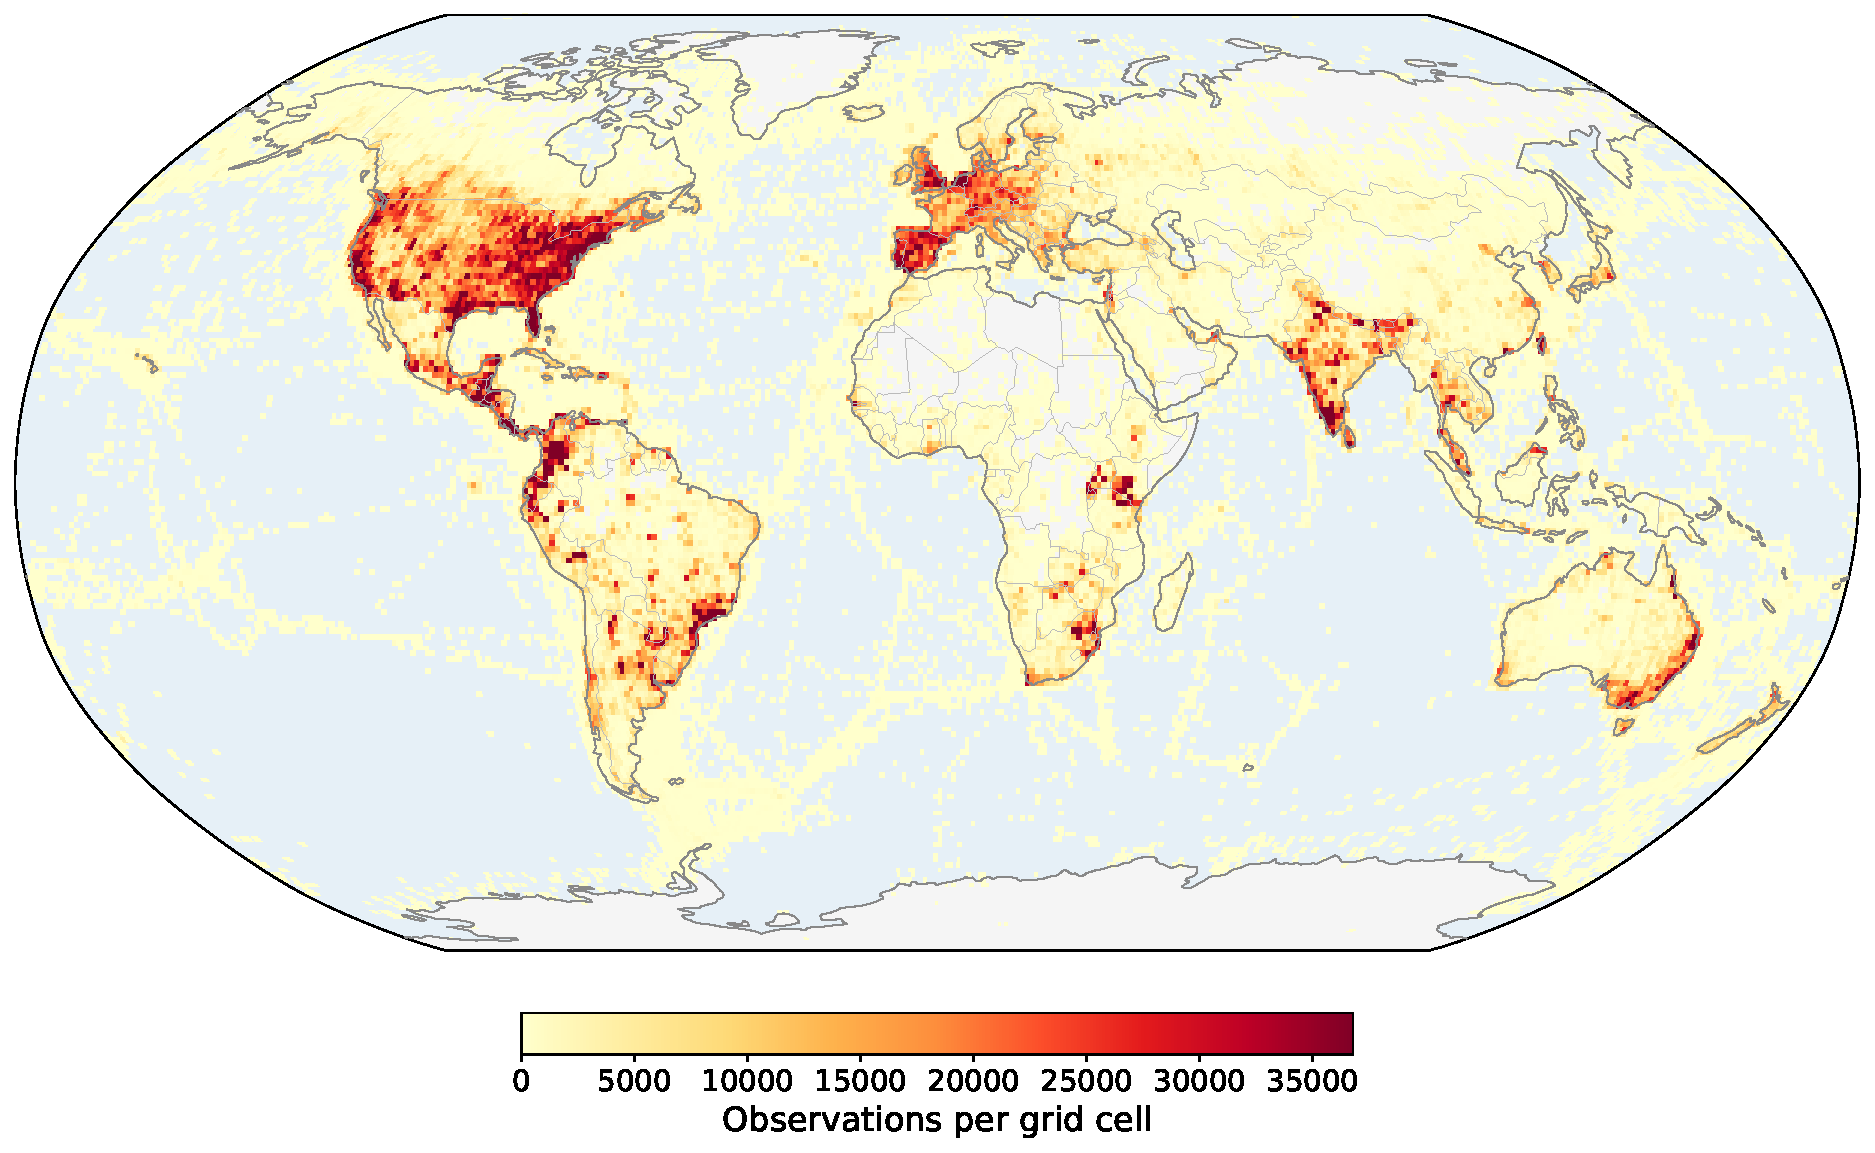
\includegraphics[width=\linewidth]{figures/observation_density.pdf}
\caption{Global observation density in the GBIF Darwin Core Archive: species-level observations per H3 cell, summed over all 48 weeks. The distribution spans four orders of magnitude and is dominated by North America and Europe (41.0\,M of 70.9\,M observations between them), while large parts of Africa, central Asia, and Amazonia carry a handful of records per cell. This imbalance is what the label propagation of Section~\ref{sec:3-3-3-label-propagation} and the density-stratified metrics of Section~\ref{sec:4-3-observation-bias-metrics} are designed to counteract.}
\label{fig:3-global-observation-d}
\end{figure}

\subsubsection{Feature Encoding}
\label{sec:3-3-2-feature-encoding}

Environmental features are encoded type-appropriately: categorical variables (e.g., land-cover class) are one-hot encoded, fractional variables (e.g., water cover) are passed through directly, and continuous variables (e.g., elevation, precipitation) are z-score standardized. Missing values are masked so that the loss function ignores cells where a given feature is unavailable (Section~\ref{sec:3-4-loss-functions}). Ocean-dominated cells can be downsampled to reduce their influence on training.

Species are identified by eBird codes (birds) or iNaturalist taxon IDs (non-birds). With vocabularies exceeding 10,000 species, labels are stored in a sparse format and expanded to full multi-label vectors during batching to keep memory usage tractable. Species observed fewer than a minimum number of times are excluded from the vocabulary.

\subsubsection{Label Propagation}
\label{sec:3-3-3-label-propagation}

Many H3 cells --- particularly outside North America and Europe --- contain too few observations to provide useful training signal, yet the species present in those regions are not absent, only unrecorded. Label propagation fills these gaps by assigning pseudo-labels from environmentally similar, well-observed cells. For each under-sampled cell the $k$ nearest neighbors in standardized environmental feature space are retrieved, subject to several ecological constraints: neighbors must share the same week (preventing seasonal leakage), lie within a geographic radius cap (preventing ecologically implausible long-range transfer), fall below an environmental-distance threshold in standardized feature space (rejecting geographically close but ecologically dissimilar neighbors), and each species may only propagate within a distance proportional to its observed range diameter from the nearest original observation, subject to a hard kilometer ceiling (preventing cosmopolitan species from filling in distant cells). The six parameters governing propagation are jointly optimized via Bayesian search (Section~\ref{sec:5-8-propagation-parameter-optimization-stage}).


\begin{algorithm}[htbp]
\centering
\begin{minipage}{\linewidth}\small\begin{verbatim}
Input: samples S = {(lat, lon, week, species_list, env_features)}
Parameters: k, max_radius, min_obs, max_spread, env_dist_max, range_cap

1  Partition samples into OBSERVED (|species_list| >= min_obs) and SPARSE
2  Standardize environmental features across all samples (zero mean, unit variance)
3  For each species s in OBSERVED samples:
4      Compute bounding-box diagonal d_s from all observations of s
5      Set max_propagation_dist_s ← min(max_spread x d_s / 2, range_cap)
6      Build a spatial index over all original observation locations of s
7  For each week w:
8      Build a KD-tree over env features of OBSERVED samples in week w
9      For each SPARSE sample q in week w:
10         Query k nearest OBSERVED neighbors in env space
11         For each neighbor n:
12             If geographic_distance(q, n) > max_radius: discard n
13             If env_distance(q, n) > env_dist_max: discard n
14         Collect candidate species from all remaining neighbors
15         For each candidate species s:
16             d ← distance from q to nearest original observation of s
17             If d > max_propagation_dist_s: discard s
18         Add surviving species to q's species list
\end{verbatim}\end{minipage}
\caption{Label propagation. Species lists are copied from well-observed cells to environmentally similar sparse cells, subject to five ecological constraints --- same week, geographic radius cap, environmental-distance gate, per-species range cap, and a kilometre ceiling on transfer distance --- each of which blocks a specific failure mode of naive nearest-neighbour imputation.}
\label{alg:1}
\end{algorithm}

Using the optimized propagation configuration (k=20, max\_radius=976 km, min\_obs=12, max\_spread=0.93, env\_dist\_max=4.99, range\_cap=1471 km), label propagation effectively fills the vast observation gaps across under-surveyed regions while preventing unrealistic pseudo-presences.

\begin{figure}[htbp]
\centering
\begin{subfigure}[t]{0.49\linewidth}
  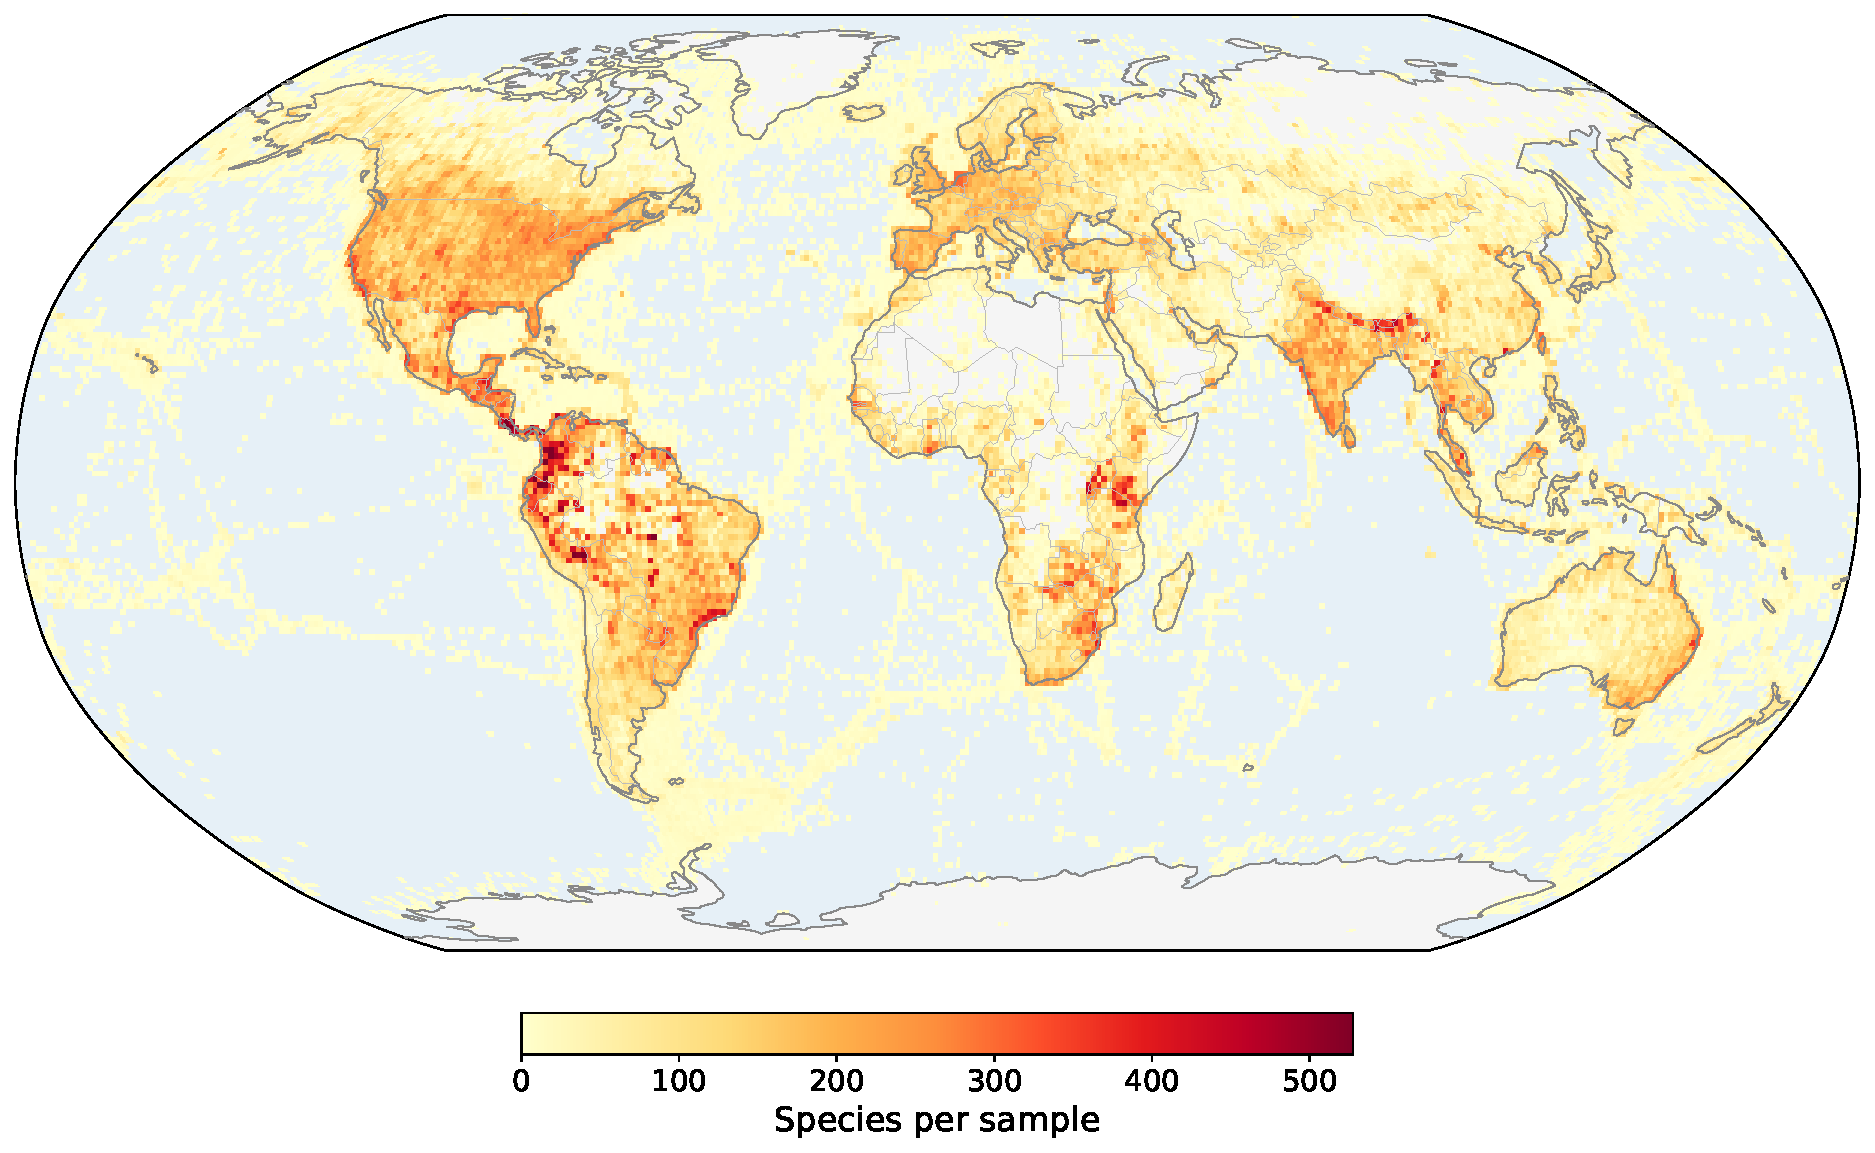
\includegraphics[width=\linewidth]{figures/label_propagation_richness_before.pdf}
  \caption{Before propagation.}
  \label{fig:4b-species-richness-per}
\end{subfigure}
\hfill
\begin{subfigure}[t]{0.49\linewidth}
  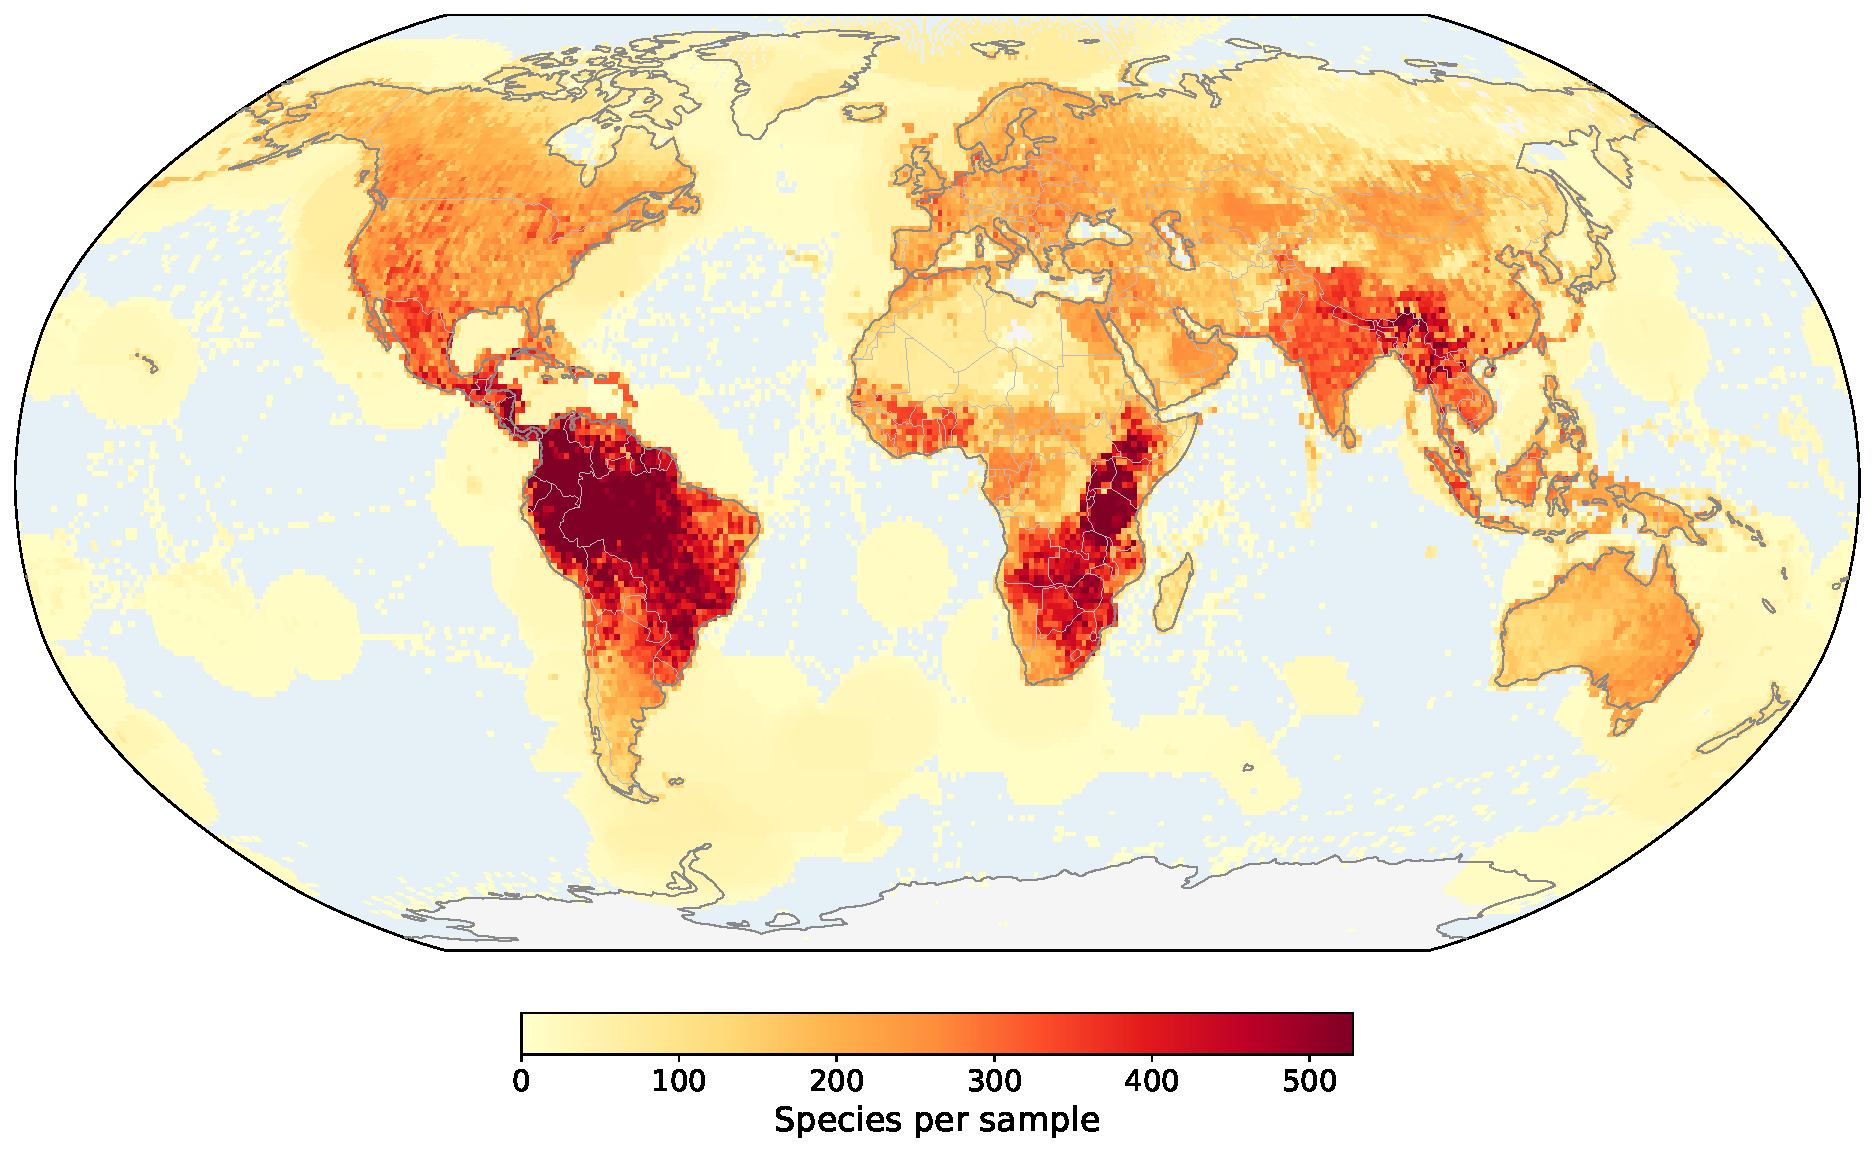
\includegraphics[width=\linewidth]{figures/label_propagation_richness_after.pdf}
  \caption{After propagation.}
\end{subfigure}
\caption{Species richness per training sample before (a) and after (b) label propagation,
using the optimized Stage H configuration ($k = 20$, radius 976\,km, sparsity threshold 12,
spread 0.93, environmental gate 4.99, range cap 1471\,km).
Before propagation the model sees rich assemblages only where observers are dense; after
it, Africa, central Asia, and Amazonia carry plausible species lists as well. This is the
single change that moves sparse-quartile mAP from 0.28 to 0.87 in the ablation
(Table~\ref{tab:1}), and it does so by supplying training signal rather than by
reweighting what was already there. Panel (b) is deliberately more generous than the
observations warrant: pseudo-labels are copies, so richness in under-sampled regions is
smoothed rather than measured. Unconstrained propagation overshoots outright --- the
sparse quartile then outscores the dense one (mAP 0.872 versus 0.719, density ratio 1.21)
--- and the ecological constraints of Stage H pull that back to 0.973. The residual cost
falls on range-restricted species, whose crisp boundaries blur (watchlist AP 0.638
$\rightarrow$ 0.535). For a filter this is the acceptable direction of error: an
over-inclusive candidate list costs a user little, whereas a species missing from the
training signal is invisible at inference.}
\label{fig:4a-species-richness-per}
\end{figure}

\begin{figure}[htbp]
\centering
\begin{subfigure}[t]{0.49\linewidth}
  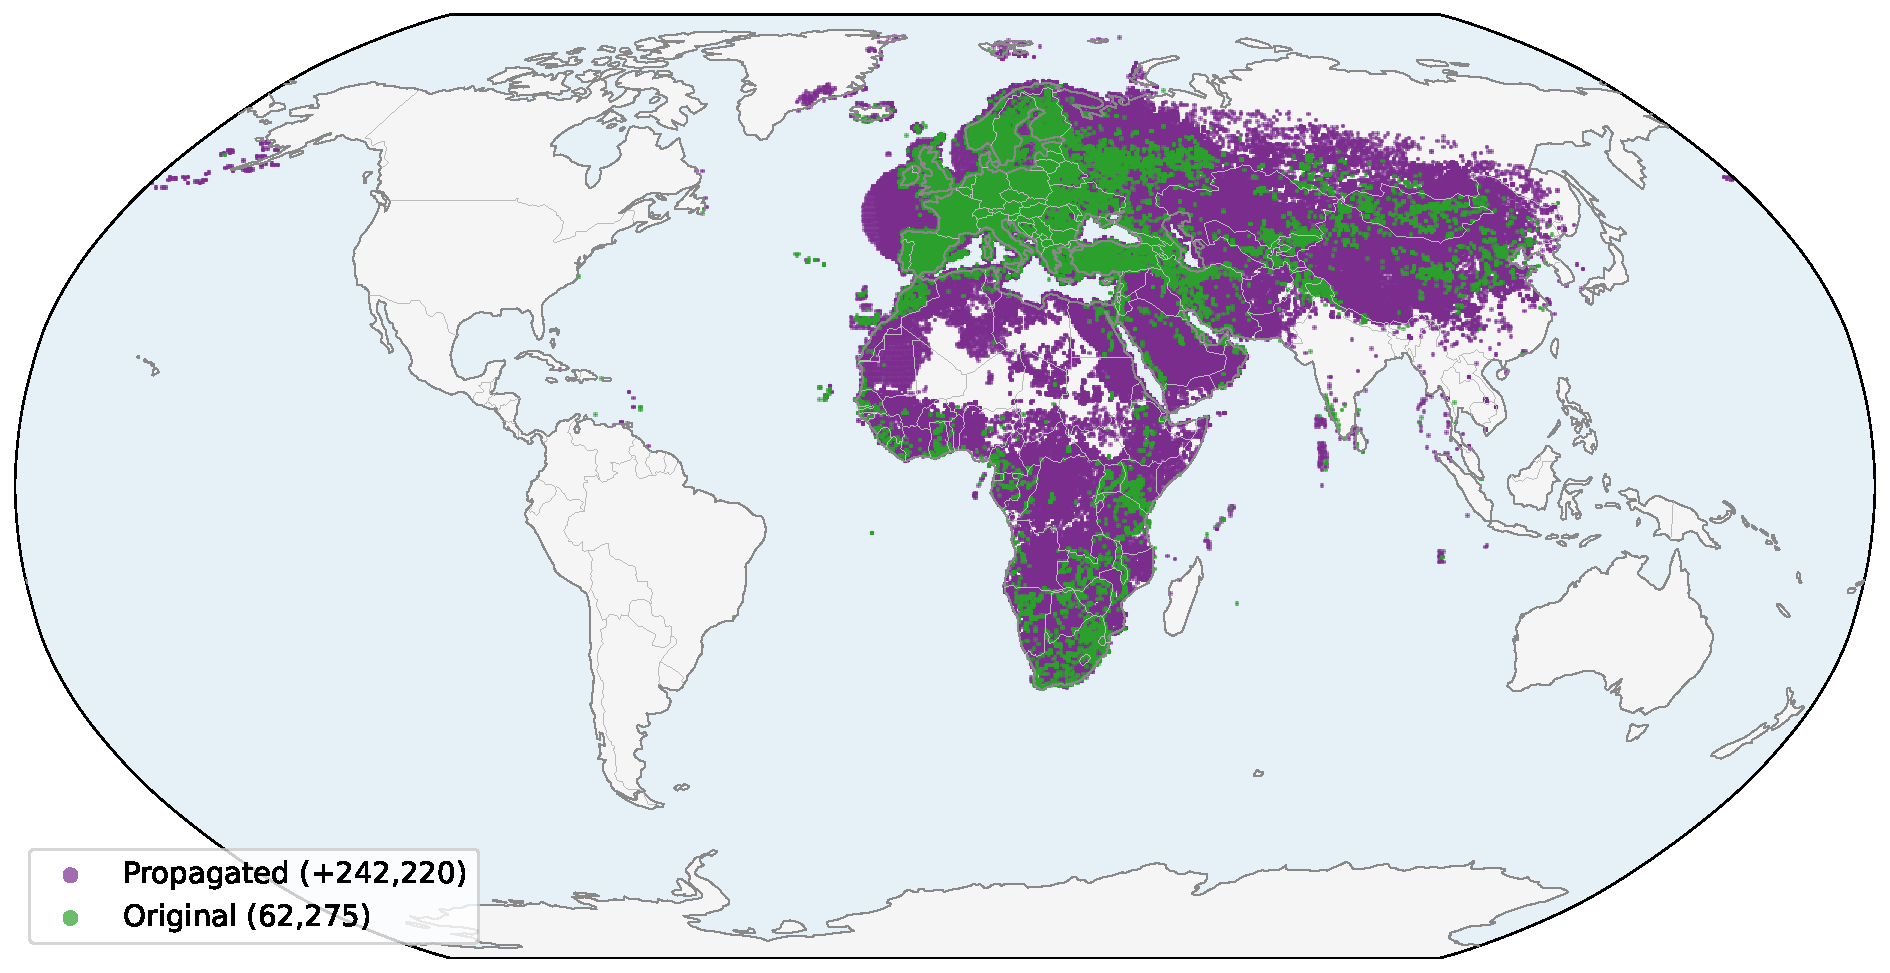
\includegraphics[width=\linewidth]{figures/label_propagation_comswi.pdf}
  \caption{Common Swift.}
  \label{fig:5b-common-hippopotamus}
\end{subfigure}
\hfill
\begin{subfigure}[t]{0.49\linewidth}
  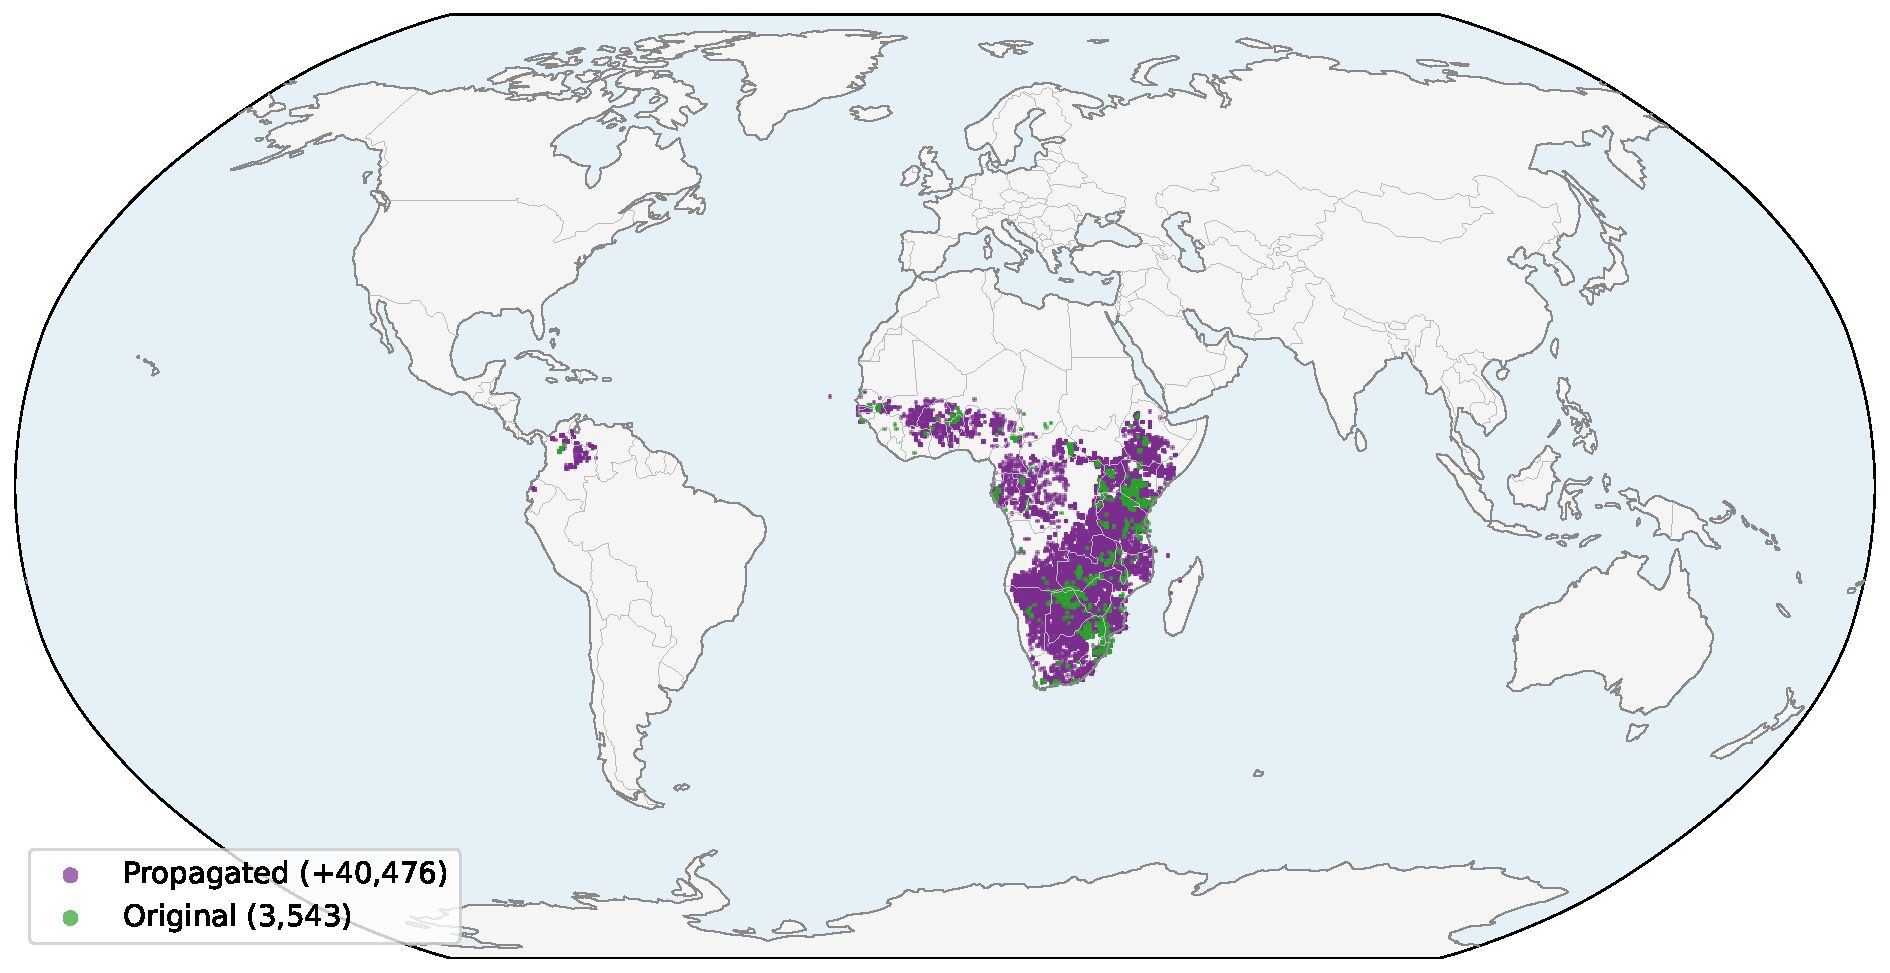
\includegraphics[width=\linewidth]{figures/label_propagation_42149.pdf}
  \caption{Common Hippopotamus.}
\end{subfigure}
\caption{Label propagation under the same optimized configuration as
Figure~\ref{fig:4a-species-richness-per}, for two species with contrasting range structure:
original observations in green, propagated pseudo-labels in purple. Common Swift (a) is a
wide-ranging Palearctic migrant whose pseudo-labels extend smoothly across under-observed
Africa and central Asia; Common Hippopotamus (b) is a range-restricted non-avian species
where the per-species range cap keeps propagation inside sub-Saharan Africa instead of
spilling into environmentally similar cells on other continents.}
\label{fig:5a-common-swift-origi}
\end{figure}

This mechanism is the single most impactful component in our ablation study (Section~\ref{sec:5-4-observation-bias-and-label-propagation-s}): enabling it increases GeoScore by 31\% (48\% once its parameters are tuned in Section~\ref{sec:5-8-propagation-parameter-optimization-stage}) and more than triples mean average precision in sparsely observed regions, because our model receives training signal for species assemblages that would otherwise be invisible.

\subsubsection{Frequency-Based Label Weights}
\label{sec:3-3-4-frequency-based-label-weights}

Citizen-science observation density varies by orders of magnitude across regions. Naive global frequency weighting would upweight common species in data-rich areas while suppressing species-rich tropical communities. We therefore compute region-normalized frequency weights: samples are partitioned into coarse geographic bins, species frequency percentiles are computed within each bin, and the maximum percentile across bins determines the final weight. This makes a species equally penalized whether it is common in Colombia or in the US, decoupling label weighting from raw observation volume. Weights are derived from pre-propagation species lists to avoid contamination by pseudo-labels.

\subsection{Loss Functions}
\label{sec:3-4-loss-functions}

Choosing the right loss function for multi-label species occurrence prediction is non-trivial. The label matrix is extremely sparse: a typical location hosts tens to low hundreds of species out of a vocabulary exceeding 10,000, so more than 99\% of labels are zero. At the same time, the zeros are unreliable --- a species scored as "absent" may simply be unrecorded, especially in under-surveyed regions. The loss must therefore handle severe class imbalance \emph{and} noisy negatives simultaneously. We implement four loss functions that represent progressively stronger assumptions about the data, allowing us to evaluate their trade-offs empirically (Section~\ref{sec:5-2-loss-function-selection-stage-a}).

The total training objective is a weighted sum of species, environmental, and (optionally) habitat terms:

\begin{equation*}
\mathcal{L}_\text{total} = w_s \cdot \mathcal{L}_\text{species} + w_e \cdot \mathcal{L}_\text{env} + w_h \cdot \mathcal{L}_\text{habitat}
\end{equation*}


\textbf{Species loss.} The four supported species loss functions span a spectrum from treating all labels as ground truth to explicitly modeling the presence-only nature of the data:

\textbf{Binary cross-entropy (BCE)} is the standard multi-label baseline. It treats every zero as a true absence and every one as a true presence, applying equal gradient pressure to all species regardless of how confident the prediction already is. Despite its simplicity, BCE is a strong default when label propagation (Section~\ref{sec:3-3-3-label-propagation}) has already filled in many of the false zeros: the propagated pseudo-labels partially compensate for the missing positive signal, and BCE's uniform gradient avoids the calibration distortions introduced by more aggressive reweighting schemes.

\textbf{Focal loss} \citep{lin2017focal} modulates the per-example gradient by a factor $(1 - p_t)^\gamma$, where $p_t$ is the predicted probability for the correct class. Well-classified examples contribute almost no gradient, concentrating learning on the hard cases. An additional per-class weight $\alpha$ balances positive and negative contributions. Focal loss was designed for dense object detection, where the ratio of background to foreground is similarly extreme; in our setting it serves the analogous purpose of preventing the overwhelming majority of zero labels from drowning out the signal from present species. However, the aggressive down-weighting can distort probability calibration: the model learns to rank species correctly but may output inflated probabilities, a phenomenon we observe as list-ratio inflation in the ablation (Section~\ref{sec:5-2-loss-function-selection-stage-a}).

\textbf{Asymmetric loss} (ASL; \citealp{ridnik2021asymmetric}) extends the focal loss idea by applying \emph{separate} focusing parameters to positive ($\gamma_+$) and negative ($\gamma_-$) terms. This recognizes that the two error types have different costs: missing a present species (false negative) is worse than hallucinating an absent one (false positive), because false negatives are unrecoverable when our model is used as a filter. Additionally, ASL introduces a probability margin $m$ that shifts the negative probability down before computing the loss:

\begin{equation*}
\mathcal{L}_\text{ASL} = -\bigl[y \cdot (1-p)^{\gamma_+} \log p + (1-y) \cdot p_m^{\gamma_-} \log(1-p_m)\bigr], \quad p_m = \max(p - m,\; 0)
\end{equation*}

When $p < m$, the negative term vanishes entirely --- the model pays no penalty for predicting a low probability for an absent species once it is already below the margin. This hard thresholding aggressively suppresses easy negatives but, like focal loss, can inflate predicted species lists.

\textbf{Assume-Negative (AN) loss} \citep{cole2023spatial} is the only function that explicitly acknowledges presence-only data. It implements the LAN-full (Location-Aware Assume Negative) strategy from SINR: at each observed location, every species not recorded in the checklist is \emph{assumed} absent. This is clearly an approximation --- some of those species are genuinely present but went undetected --- so positive observations are up-weighted by a factor $\lambda$ (default 4) to compensate. For computational efficiency with a \textasciitilde{}12K-species vocabulary, only a random subset of negative species is evaluated per sample; the sampled loss is rescaled to provide an unbiased approximation of the full-vocabulary expectation. Optional label smoothing softens the binary targets slightly, preventing overconfident predictions.

\textbf{Environmental loss.} The environmental head is trained with masked mean squared error: the loss is computed only over cells where the Earth Engine target is available, ignoring cells with missing data. The environmental weight $w_e$ controls how strongly the regression objective shapes the shared encoder representation. Setting it too high biases the encoder toward environmental reconstruction at the expense of species discrimination; setting it to zero removes the auxiliary signal entirely, relying on the encoder to discover environmental structure implicitly from species co-occurrence alone --- which, as the ablation shows (Section~\ref{sec:5-3-model-capacity-and-representation-mode-s}), large models are capable of.

\textbf{Habitat loss.} When the habitat head is active, the same species loss is applied directly to the habitat head's logits before gating. This gives the habitat pathway an independent learning signal: without it, the habitat head would receive gradients only through the gate, which is initialized to strongly favor the direct head, creating a chicken-and-egg problem where the habitat head cannot learn because it receives almost no gradient, and the gate cannot open because the habitat head has not yet learned.

\subsection{Training Procedure}
\label{sec:3-5-training-procedure}

Our model is trained with AdamW \citep{loshchilov2019decoupled} using decoupled weight decay. The learning rate follows a cosine annealing schedule with a three-epoch linear warmup. Gradient norms are clipped to prevent training instabilities. Training uses automatic mixed precision on CUDA GPUs: forward passes run in FP16 for roughly double the throughput, while loss computation and parameter updates remain in full precision.

\textbf{Location-based splitting.} To prevent spatial data leakage --- a concern raised by \citet{kellenberger2026performance} --- the train/validation split operates at the level of H3 cells, not individual samples. All 48 weekly samples from a given cell go entirely into either the training or the validation set, so our model is always evaluated on locations it has never seen. Additionally, entire well-surveyed geographic regions can be withheld from training for holdout evaluation: we define five such regions (US Northwest, BeNeLux, Great Britain, California, and Japan), chosen for high eBird observer density and therefore reliable ground-truth labels.

\textbf{Early stopping.} Training halts when the composite GeoScore metric (Section~\ref{sec:4-1-geoscore}) does not improve for a configurable number of epochs. The best-scoring checkpoint is retained.

\subsection{Hyperparameter Search}
\label{sec:3-6-hyperparameter-search}

An automated Bayesian search \citep{akiba2019optuna} optimizes GeoScore over up to 23 parameters spanning loss function selection and tuning, model capacity (scale factor, harmonic counts), task weighting, data augmentation, frequency weighting, and label propagation. The search uses TPE sampling with median pruning for early termination of unpromising trials. Selective tuning --- fixing some parameters while searching over others --- allows efficient exploration of individual design dimensions, which we exploit in the staged ablation study described in Section~\ref{sec:5-experiments-and-results}

\subsection{Export and Deployment}
\label{sec:3-7-export-and-deployment}

Trained models are exported to ONNX, TensorFlow Lite (FP32, FP16, and INT8 dynamic-range quantization), and TensorFlow SavedModel. The critical export format is FP16, which compresses the production model (\textasciitilde{}12K species, scale 0.75) to approximately 7 MB --- well within the <10 MB budget for mobile apps and embedded acoustic sensors. INT8 dynamic-range quantization reduces this further to \textasciitilde{}4 MB. This is essential to our model's intended use case: BirdNET Analyzer, the BirdNET mobile app, Haikubox, and BirdWeather all run on resource-constrained platforms where a multi-gigabyte model would be impractical.

Inputs and outputs retain full precision even in the FP16 model, preserving coordinate and probability accuracy. After each conversion, an automated validation compares outputs against the PyTorch reference across diverse locations and weeks, confirming negligible differences. The architectural precautions described above --- bounded FiLM gamma, safe LayerNorm epsilon --- are what make this agreement possible: without them, half-precision quantization would introduce cascading numerical errors through the encoder stack.


\section{Evaluation}
\label{sec:4-evaluation}

A species distribution model must not only rank species correctly at well-surveyed locations but also generalize to poorly observed regions and maintain calibrated predictions --- a model that assigns high probability to every species achieves perfect recall but is useless as a filter. We therefore evaluate along three complementary axes: standard classification quality, robustness to observation bias, and performance on rare and range-restricted species. These are combined into a single composite metric, GeoScore, that serves as the optimization target during training and hyperparameter search.

\subsection{GeoScore}
\label{sec:4-1-geoscore}

GeoScore is a weighted average of seven components, each normalized to $[0, 1]$ where higher is better. It is designed to penalize a model that excels on one axis (e.g., raw ranking) while failing on another (e.g., predicting far too many species per location). The components and their weights are:

\begin{table}[htbp]
\centering
\small
\begin{tabularx}{\linewidth}{llL}
\toprule
Component & Weight & What it measures \\
\midrule
mAP & 0.20 & Mean per-sample average precision: how well the model ranks present species above absent ones across the full vocabulary. \\
F1 @ 10\% & 0.20 & Micro-averaged F1 score at a 10\% probability threshold --- a direct measure of the quality of the predicted species list at a practical operating point. \\
List ratio @ 10\% & 0.15 & Mean ratio of predicted to true species count at 10\% threshold. Transformed via exp($-|$log r$|$), which penalizes both over-prediction (r $\gg$ 1) and under-prediction (r $\ll$ 1) symmetrically on a log scale, with a perfect score of 1.0 at r = 1. \\
Watchlist AP & 0.10 & Mean average precision across a curated set of 18 endemic and restricted-range species (Section~\ref{sec:4-4-watchlist-species}), ensuring the model does not sacrifice rare-species performance for aggregate accuracy. \\
Holdout mAP & 0.10 & mAP computed exclusively on geographically held-out regions (Section~\ref{sec:3-5-training-procedure}), testing whether the model generalizes to areas entirely absent from training. \\
Density ratio & 0.20 & Ratio of mAP in the sparsest observation-density quartile to mAP in the densest quartile, transformed via min(r, 1/r) so that both under- and over-correction are penalized symmetrically (peak at 1.0). A score near 1.0 means the model performs equally well regardless of how heavily a region has been surveyed. This is the single largest-weighted component because observation-bias robustness is a central goal. \\
Pred--density corr & 0.05 & Pearson correlation between observation density and the number of species predicted at 10\% threshold, transformed as max(0, 1 $-$ $|$r$|$). A model that predicts more species in heavily birded areas --- regardless of true richness --- will score poorly here. \\
\bottomrule
\end{tabularx}
\end{table}

Components that are unavailable (e.g., holdout mAP when no holdout regions are defined) are dropped and the remaining weights renormalized. This makes GeoScore comparable across runs with different evaluation configurations.

The weighting reflects our priorities: ranking quality (mAP + F1) and bias robustness (density ratio + pred--density correlation) each receive 40\% of the total weight between them, list calibration receives 15\%, and the remaining 20\% is split between geographic generalization and rare-species coverage. These weights were set before the ablation study and held fixed throughout.

\subsection{Standard Classification Metrics}
\label{sec:4-2-standard-classification-metrics}

\textbf{Mean average precision (mAP)} is computed per sample: for each validation location $\times$ week, we rank all $S$ species by predicted probability, compute the average precision of the true positive set, and average across samples. mAP measures ranking quality independent of any threshold --- it answers how well the model separates present from absent species.

\textbf{Top-$k$ recall} at $k = 10$ and $k = 30$ measures the fraction of truly present species that appear in the model's $k$ highest-scoring predictions. This is directly relevant to the acoustic-filtering use case, where the model proposes a short candidate list and the classifier searches only among those species.

\textbf{Threshold-based metrics.} At probability thresholds of 5\%, 10\%, and 25\%, we compute micro-averaged precision, recall, and F1. The 10\% threshold is the primary operating point --- it is the threshold at which the BirdNET app and related tools decide whether a species is plausible at a given location and week. We also compute the \textbf{mean list length} (how many species exceed the threshold per sample) and the \textbf{list ratio} (predicted list length divided by true list length), which reveals whether the model tends to over- or under-predict species counts.

\subsection{Observation Bias Metrics}
\label{sec:4-3-observation-bias-metrics}

Citizen-science data is concentrated in wealthy, accessible, English-speaking regions. A model that simply memorizes observation density --- predicting many species in New York and few in Amazonia --- would achieve respectable mAP despite having learned nothing about ecology. We measure susceptibility to this failure mode with two metrics.

\textbf{Density-stratified mAP.} Validation samples are split into quartiles by the observation density of their H3 cell. We report mAP separately for the sparsest quartile ($\mathrm{mAP}_\text{sparse}$) and densest quartile ($\mathrm{mAP}_\text{dense}$), and their ratio: a model with $\mathrm{mAP}_\text{sparse}$ / $\mathrm{mAP}_\text{dense}$ $\approx 1$ performs equally well in under-surveyed and heavily surveyed regions. Our ablation shows this ratio ranges from 0.33 (strong bias) to 1.21 (slight over-correction) depending on whether label propagation is active (Section~\ref{sec:5-4-observation-bias-and-label-propagation-s}).

\textbf{Prediction--density correlation.} We compute the Pearson correlation between observation density and the number of species predicted above the 10\% threshold across all validation samples. A high positive correlation means the model predicts richer communities in data-rich regions regardless of true species richness --- the hallmark of a model that has absorbed sampling bias into its predictions rather than filtering it out.

\subsection{Watchlist Species}
\label{sec:4-4-watchlist-species}

To ensure that aggregate metrics do not mask failures on conservation-relevant species, we track per-species average precision for a curated watchlist of 18 endemic and restricted-range species drawn from three island archipelagos and a small set of otherwise restricted-range or critically endangered taxa:

\begin{itemize}
  \item \textbf{Hawaiian endemics} (6 species): Hawaiian Goose, Hawaiian Hawk, Hawaii Elepaio,
Apapane, Iiwi, Hawaii Amakihi --- all confined to the Hawaiian Islands, with several classified as Endangered or Vulnerable.
  \item \textbf{New Zealand endemics} (6 species): Kea, North Island Brown Kiwi, South Island
Takahe, Rifleman, Tui, North Island Kokako --- flightless and restricted-range species that test whether the model can resolve island-scale boundaries.
  \item \textbf{Galápagos endemics} (3 species): Galápagos Hawk, Galápagos Rail, Galápagos
Petrel --- extremely restricted ranges that demand precise spatial predictions.
  \item \textbf{Other restricted-range and critically endangered} (3 species): Kagu (New Caledonia),
California Condor, Whooping Crane --- species with tiny populations and ranges confined to a few known sites.
\end{itemize}

The watchlist mean AP is the unweighted average across all species with at least one positive sample in the validation set. A model that achieves high aggregate mAP but low watchlist AP has learned to predict common species while ignoring the rarest ones --- a failure mode with direct conservation implications.


\section{Experiments and Results}
\label{sec:5-experiments-and-results}

We evaluate our model through a staged ablation study comprising 46 grid-search experiments (Stages A--G) plus 60 Bayesian propagation-parameter optimization trials (Stage H). Each grid stage isolates one design dimension, selects a single winner by GeoScore, and carries that configuration forward to the next stage. Stage H then optimizes the six propagation hyperparameters using automated search. This greedy, sequential protocol is more sample-efficient than full factorial search while still quantifying the marginal contribution of each factor. Table~\ref{tab:1} summarizes the stage winners; full per-run tables are provided in Appendix~\ref{sec:B-full-ablation-results-tables}.

\subsection{Experimental Setup}
\label{sec:5-1-experimental-setup}

All experiments share a common base configuration: batch size 1024, 20 training epochs, AdamW with cosine-annealed learning rate ($10^{-3}$), patience-5 early stopping on GeoScore, location-based train/validation split, no yearly encoding, and a minimum species-observation threshold of 50. Each stage varies one or two factors atop the previous winner's configuration. Holdout regions were not used during ablation; the holdout mAP component of GeoScore is therefore absent and the remaining weights are renormalized. We report the best-epoch GeoScore for each run.


\begin{table}[!ht]
\centering
\caption{Stage winners: the best configuration carried forward from each ablation stage. Density ratio is mAP in the sparsest observation quartile divided by mAP in the densest, so values near 1.0 indicate spatially unbiased predictions; LR@10\% is the list ratio at the 10\% probability threshold, where lower is better calibrated. The single largest jump is at Stage C, where enabling label propagation raises GeoScore from 0.431 to 0.564 and moves the density ratio from 0.332 to 1.212 --- the model stops being systematically better in well-surveyed regions.}
\label{tab:1}
\small
\resizebox{\linewidth}{!}{%
\begin{tabular}{llrrrrrrrrr}
\toprule
Stage & Description & GeoScore & mAP & mAP (sparse) & mAP (dense) & F1@10\% & LR@10\% & Watchlist AP & Density Ratio & pred--density r \\
\midrule
A & BCE, light label smoothing & 0.422 & 0.543 & 0.276 & 0.847 & 0.511 & 6.43 & 0.701 & 0.33 & 0.797 \\
B & Scale 2.0, coordinate-only & 0.431 & 0.547 & 0.282 & 0.849 & 0.519 & 6.06 & 0.730 & 0.33 & 0.795 \\
C & No env task, propagation on & 0.564 & 0.694 & 0.872 & 0.719 & 0.499 & 4.72 & 0.638 & 1.21 & 0.831 \\
D & 8 spatial + 8 temporal harmonics & 0.566 & 0.698 & 0.877 & 0.720 & 0.509 & 4.45 & 0.612 & 1.22 & 0.827 \\
E & Jitter on, yearly off & 0.566 & 0.697 & 0.876 & 0.719 & 0.505 & 4.55 & 0.635 & 1.22 & 0.830 \\
F & Observation cap at 5000 & 0.388 & 0.207 & 0.344 & 0.194 & 0.169 & 1.55 & 0.415 & 1.78 & 0.531 \\
\textbf{H} & \textbf{Optimized propagation} & \textbf{0.638} & \textbf{0.781} & \textbf{0.809} & \textbf{0.831} & \textbf{0.602} & \textbf{3.48} & \textbf{0.535} & \textbf{0.973} & \textbf{0.870} \\
\bottomrule
\end{tabular}
}
\end{table}

\subsection{Loss Function Selection (Stage A)}
\label{sec:5-2-loss-function-selection-stage-a}

Our first question is which loss function best suits a multi-label, presence-only prediction task with over 10,000 species. We hypothesize that losses explicitly designed for class imbalance or presence-only data --- Asymmetric Loss (ASL), Focal, and Assume-Negative (AN) --- should outperform standard BCE, because the label matrix is >99\% zeros and the zeros are unreliable (an unrecorded species may be present but undetected). We test three settings per family (conservative, default, aggressive) for 12 runs total, all at the reference model scale (1.0) with a moderate environmental task weight (0.1).

The comparison is unambiguous: BCE is the strongest of the four families. All 12 runs achieve nearly identical mean average precision (mAP 0.536--0.544), confirming that ranking ability is robust to loss choice. Calibration, however, varies by orders of magnitude. BCE produces a list ratio at the 10\% threshold (LR@10\%) of approximately 6 --- the model predicts roughly six times more species than are truly present, a reasonable starting point for a permissive filter. ASL aggressively down-weights easy negatives, which paradoxically \emph{inflates} predicted lists: its most aggressive setting yields LR@10\% = 979, meaning the model predicts nearly every species at every location. Focal loss shows the same pattern at reduced severity. AN loss, which explicitly models presence-only data through up-weighted positives and negative sampling, is the second-best family but still trails BCE by roughly 11\% in GeoScore. The differences are entirely in calibration, not ranking --- an important consideration for multi-species SDMs, where the raw probability values matter as much as their ordering.

BCE with light label smoothing (0.05) achieves the highest GeoScore (0.422) and a watchlist AP of 0.701. We carry this configuration forward.

\subsection{Model Capacity and Representation Mode (Stage B)}
\label{sec:5-3-model-capacity-and-representation-mode-s}

Given BCE as the loss baseline, we next ask whether environmental auxiliary tasks or the habitat head improve performance, and how these interact with model scale. The reasoning is as follows. A larger model has more capacity to memorize spatial patterns, which may substitute for explicit environmental guidance. Conversely, a small model might benefit from the inductive bias of predicting environmental features as an auxiliary task, since that forces the shared encoder to learn ecologically meaningful representations rather than arbitrary spatial correlations. The habitat head, which routes environment predictions through a secondary species classifier, makes this connection explicit.

We cross three model scale factors (0.5$\times$, 1.0$\times$, 2.0$\times$) with three representation modes --- coordinate-only (no environmental task), environmental auxiliary (moderate regression weight), and environment plus habitat head --- yielding nine runs. The pattern is consistent: model scale matters more than either representation choice. Every metric improves monotonically from the smallest to the largest model within each mode (GeoScore: 0.408 $\rightarrow$ 0.431 for coordinate-only), and the coordinate-only mode wins at scale 2.0. The environmental auxiliary task adds no signal that a sufficiently large model cannot learn on its own: at the largest scale, the environmental mode achieves slightly higher raw mAP (0.552 vs 0.547) but at the cost of worse calibration, netting a lower GeoScore. The habitat head likewise provides no benefit --- it adds parameters and architectural complexity without improving any metric. Watchlist AP follows the same pattern: the largest coordinate-only model achieves the best endemic species performance (0.730), suggesting that big models learn restricted ranges better even without explicit environmental structure.

This finding has a simple interpretation: when the model is large enough, the mapping from (latitude, longitude) to species occurrence implicitly captures all the environmental gradients that matter. Elevation, climate, and land cover vary smoothly across space, and a 7M-parameter network with multi-harmonic coordinate encoding has ample capacity to approximate those gradients without being told they exist. We carry forward the largest model scale with no environmental auxiliary task.

\subsection{Observation Bias and Label Propagation (Stage C)}
\label{sec:5-4-observation-bias-and-label-propagation-s}

This is the central experiment of the ablation. Citizen-science data is concentrated in wealthy, accessible regions: North America averages 688 observations per H3 cell versus 152 for Africa. A naive model will learn to predict many species in New York and few in Amazonia --- not because of ecology, but because of sampling effort. We test two mechanisms for mitigating this bias: the environmental auxiliary task at four weight levels (zero through heavy), which encourages the encoder to learn physical environment rather than observer density, and label propagation, which imputes species lists from well-observed cells to nearby under-observed ones using environmental similarity.

Label propagation is, by a wide margin, the single most impactful factor in our entire ablation. Enabling it raises GeoScore from approximately 0.43 to 0.56 --- a 31\% improvement that dwarfs every other intervention. The mechanism is a structural redistribution of performance: mAP in the sparsest observation-density quartile jumps from 0.28 to 0.87 (+210\%), while mAP in the densest quartile drops from 0.85 to 0.72 ($-$15\%). The density ratio flips from 0.33 (dense regions dominate) to 1.21 (sparse regions slightly outperform dense). In other words, before propagation the model is roughly three times more accurate in the best-surveyed quartile than in the least-surveyed one; afterwards the two are comparable.

The environmental auxiliary task, by contrast, has no measurable effect. Across all four weight levels, GeoScore varies by less than 1\% in both propagation regimes. This confirms the intuition from Stage B: the model already learns environmental gradients implicitly from species co-occurrence, and adding an explicit regression target provides no additional signal.

There is a cost. Watchlist AP drops from 0.724 to 0.638 when propagation is enabled, because propagated pseudo-labels blur the boundaries of highly range-restricted species. A Hawaiian endemic that occurs on a single island may receive propagated labels on neighboring islands, diluting the model's ability to resolve its precise range. This tradeoff is inherent to the method: propagation helps where data are sparse, but those are precisely the regions where range boundaries are hardest to impute correctly.

\subsection{Encoding Resolution, Augmentation, and Training Choices (Stages D--E)}
\label{sec:5-5-encoding-resolution-augmentation-and-tra}

With the architectural and data-pipeline decisions settled, we sweep the remaining engineering parameters. The harmonic encoding resolution (Stage D: 2, 4, or 8 spatial harmonics crossed with 4 or 8 temporal harmonics, six runs) and augmentation/temporal choices (Stage E: coordinate jitter on/off crossed with yearly encoding on/off, four runs) produce markedly smaller effects than the earlier stages.

All six harmonic configurations span less than 0.5\% in GeoScore (0.562--0.566). Higher spatial harmonics provide a slight edge --- they capture finer geographic boundaries (e.g., island coasts, mountain ranges) --- and the maximum setting (eight harmonics each for coordinates and week) wins narrowly. The effect is so small because label propagation has already smoothed the target distributions across neighboring cells, reducing the model's need for sharp spatial resolution in its encoding.

Similarly, coordinate jitter and yearly encoding produce GeoScore differences below 0.3\%. Jitter provides a marginal regularization benefit (+0.1\% GeoScore) by preventing the model from overfitting to exact H3 cell centroids. Yearly encoding, which adds a linear time component alongside the cyclical week encoding, consistently hurts: the 48-week cycle already captures seasonal phenology, and adding a continuous year dimension introduces noise without improving generalization. We carry forward coordinate jitter enabled and yearly encoding disabled (GeoScore 0.566, mAP 0.697).

\subsection{Observation Capping and Vocabulary Scaling (Stages F--G)}
\label{sec:5-6-observation-capping-and-vocabulary-scali}

The final grid stages test two data-level interventions. Stage F caps the maximum observations per species (500, 5000, or 50000), asking whether limiting dominant species (e.g., House Sparrow at \textasciitilde{}480K observations) improves performance for rarer taxa. Stage G restricts the species vocabulary to subsets of 10, 100, 1000, and 5000 species to measure how multi-species training scales.

Observation capping does not help. Capping at 5000 cuts GeoScore from 0.566 to 0.388 --- a 31\% degradation --- because species discrimination collapses (mAP: 0.697 $\rightarrow$ 0.207). While the density ratio improves from 1.22 to 1.78, this over-corrects past the ideal balance of 1.0, and GeoScore correctly penalizes the over-correction: a density ratio of 1.78 scores the same as 0.56, reflecting the model's failure to distinguish dense- and sparse-region assemblages. Capping at 50,000 preserves reasonable mAP (0.521) with a modest GeoScore penalty (0.457). Capping at 500 collapses entirely (GeoScore 0.092). The fundamental issue is that capping achieves spatial uniformity by making the model \emph{worse everywhere}, not by making it better in sparse regions. Constrained label propagation (Stage H) achieves the same spatial-balance goal far more effectively.

The vocabulary scaling study confirms that model capacity is not limiting. Within the observation-capped G regime, GeoScore at 5000 species (0.434) exceeds the full vocabulary at 11,827 species (0.388), and the monotonic mAP decrease with vocabulary size (0.879 at 10 $\rightarrow$ 0.207 at 11,827) reflects the combinatorial difficulty of multi-label classification, not model insufficiency. This suggests that expanding the vocabulary to 20,000+ species would require more training data, not a bigger model.

\subsection{Hypothesis Resolution}
\label{sec:5-7-hypothesis-resolution}

Table~\ref{tab:2} summarizes the nine hypotheses motivating the ablation and their outcomes. Five are confirmed outright, three are confirmed with qualifications that matter for deployment, and one --- the expectation that an explicit habitat head would aid transfer to under-observed regions --- is refuted.


\begin{table}[!ht]
\centering
\caption{Resolution of the nine ablation hypotheses. The two refuted expectations are instructive: an explicit habitat head does not improve transfer to under-observed regions, and larger models do not concentrate their gains in dense regions once propagation is active.}
\label{tab:2}
\small
\begin{tabularx}{\linewidth}{lLL}
\toprule
\# & Hypothesis & Result \\
\midrule
H1 & Environmental auxiliary task improves sparse-region robustness & \textbf{No.} Environmental task weight has no effect in either propagation regime. \\
H2 & Label propagation helps under-observed regions & \textbf{Yes.} The single most impactful factor: +31\% GeoScore, +210\% sparse-region mAP. \\
H3 & Habitat head improves transfer to low-observation regions & \textbf{No.} Adds complexity without benefit at any model scale. \\
H4 & Larger models need environmental guidance for robust transfer & \textbf{Partial.} Larger models help uniformly, but do not need env guidance. \\
H5 & Loss function affects calibration more than ranking & \textbf{Yes.} All losses achieve similar mAP; calibration varies by 100$\times$. \\
H6 & Coordinate jitter improves generalization & \textbf{Weakly.} Marginal positive signal (<0.5\%), not decisive. \\
H7 & Yearly encoding captures inter-annual trends & \textbf{No.} Consistently hurts; cyclical week encoding suffices. \\
H8 & Observation capping reduces spatial bias & \textbf{Mixed.} Improves equity metrics but destroys species discrimination. \\
H9 & Model capacity limits performance at large vocabularies & \textbf{No.} Full vocabulary matches 5000-species performance; data sparsity is the bottleneck. \\
\bottomrule
\end{tabularx}
\end{table}

\subsection{Propagation Parameter Optimization (Stage H)}
\label{sec:5-8-propagation-parameter-optimization-stage}

The initial propagation parameters used in early stages were chosen conservatively: few neighbors, a broad geographic radius, and a low observation threshold, with no explicit ecological constraints on which cells could receive propagated labels. Stage H optimizes six propagation parameters to maximize GeoScore while maintaining ecological realism. Beyond the three original parameters (neighbor count, search radius, and minimum observation threshold), we explicitly introduce ecological safeguards: an environmental-distance gate that rejects candidates whose standardized environmental profile differs too greatly from the target cell, and a per-species range cap that limits propagation distance from the nearest original observation of that species. A range-spread factor, which scales each species' observed range diameter, provides a sixth degree of freedom.

An initial exploratory search exposed a failure mode of the objective itself: without explicit constraints, the optimizer pushes propagation toward extreme distances because doing so inflates the spatial-balance metrics, producing range expansions with no ecological basis. To counteract this, the final tuning run strictly bounds expansion by measuring distance from the nearest true observation, allowing propagation for migratory species without unbounded inflation.

The optimized configuration (k=20, max radius=976 km, min obs=12, max spread=0.93, env dist max=4.99, range cap=1471 km) yields the best discrimination in the study (mAP 0.781) together with near-balanced spatial performance (density ratio 0.973) and the highest overall GeoScore (0.638). This confirms that label propagation is most effective when aggressively filling sparse gaps but strictly fenced by nearest-observation range limits and environmental matching.

\subsection{Recommended Configuration}
\label{sec:5-9-recommended-configuration}

The ablation establishes a clear hierarchy of design choices: label propagation dominates (+31\% GeoScore when enabled, a further +13\% once its parameters are constrained and tuned in Stage H), followed by model scaling and loss function choice.

For the production model, we recommend using the Stage H final optimized propagation parameters. The ablation favors the largest scale tested (2.0), but at \textasciitilde{}47M parameters it would exceed 40 MB in FP16, and even scale 1.0 produces a \textasciitilde{}14 MB FP16 model that misses the <10 MB target for mobile and embedded deployment. Scale 0.75 (3.8M parameters, \textasciitilde{}7 MB FP16) retains most of the capacity benefit of scale 1.0 while fitting comfortably on mobile phones and embedded acoustic sensors; scale 2.0 at \textasciitilde{}47M parameters would exceed 40 MB in FP16. The environmental auxiliary task can optionally be enabled during training as it adds no measurable cost to species prediction and may prove useful for downstream habitat representation learning.

The central finding is that ecologically constrained label propagation --- bounded relative to the nearest known observations and filtered by local environment --- affects model performance more than the choice of loss function or any architectural variant we tested.


\section{Comparison with eBird Status and Trends}
\label{sec:6-comparison-with-ebird-status-and-trends}

To assess whether the geomodel produces ecologically plausible spatial and temporal patterns, we compare its occurrence predictions against eBird Status and Trends (S\&T) 2023 median abundance surfaces \citep{fink2024ebird}. The two systems differ fundamentally: S\&T models each species independently using adaptive spatio-temporal ensembles with effort covariates; our model uses a single shared network for all species with no environmental inputs at inference. Both ultimately derive from eBird checklists, so this comparison is not an independent validation in the strict sense. However, because S\&T applies a fundamentally different modeling methodology and is curated by domain experts, agreement between the systems serves as a meaningful sanity check on range geometry and seasonal phenology, while disagreement highlights where the coordinate-only approach diverges from covariate-driven predictions.

\subsection{Methodology}
\label{sec:6-1-methodology}

We compare 10 species spanning diverse migration strategies and geographic extents: long-distance migrants (Amur Falcon, Bobolink, Common Swift, Northern Wheatear), medium-distance migrants (European Bee-eater, Ruby-throated Hummingbird, Rufous Hummingbird, Wilson's Warbler), and residents (Blue-and-yellow Macaw, Northern Cardinal). Each species is evaluated at two contrasting time points --- week 1 (early January) and week 26 (mid-July) --- to capture both breeding and non-breeding distributions.

Both prediction surfaces are projected onto a shared 0.5\textdegree{} global latitude-longitude grid (360 $\times$ 720 = 259,200 cells). Because S\&T outputs relative abundance while our model outputs occurrence probability, direct value comparison is not meaningful; instead, both are converted to binary presence/absence. S\&T cells with any positive abundance are treated as present; geomodel predictions are binarized at a single global probability threshold that maximizes mean F1 across all 20 species-week pairs (optimum = 0.167). We round down to \textbf{$t = 0.15$} --- within 0.3\% of the optimal mean F1 --- because a round number is easier to communicate and apply in practice. This single-threshold approach reflects realistic usage where per-species calibration data is unavailable. All metrics are computed only within the S\&T valid mask, so the geomodel is not penalized for predicting in regions S\&T does not cover.

We report five metrics: Jaccard index (intersection-over-union of the two binary ranges), precision and recall (measuring over- and under-prediction relative to S\&T), F1 (harmonic mean), and AUC (ROC area under curve, using the geomodel's continuous probability against S\&T binary presence --- a threshold-free discrimination measure).

\subsection{Results}
\label{sec:6-2-results}

Table~\ref{tab:3} reports all five metrics for the 20 species--week pairs, together with the
means across pairs. Two summary observations frame the discussion that follows: discrimination is uniformly strong (AUC below 0.95 in only one of twenty comparisons), while
threshold-dependent overlap varies widely across species and seasons, from 0.199 to 0.795 in
Jaccard. Section~\ref{sec:6-3-interpretation} takes up both patterns in turn.

\begin{table}[!ht]
\centering
\caption{Range overlap with eBird Status and Trends on a 0.5\textdegree{} grid at threshold 0.15 (production model, scale 0.75). Recall exceeds precision in 18 of 20 comparisons, which is the model over-predicting at range margins rather than missing core range --- the preferable error direction for a filter. AUC, which needs no threshold, stays above 0.94 everywhere except Northern Wheatear in July.}
\label{tab:3}
\small
\begin{tabular}{llrrrrr}
\toprule
Species & Week & Jaccard & Precision & Recall & F1 & AUC \\
\midrule
Amur Falcon & Week 1 (Jan) & 0.709 & 0.727 & 0.966 & 0.830 & 0.994 \\
Amur Falcon & Week 26 (Jul) & 0.648 & 0.870 & 0.718 & 0.787 & 0.992 \\
Blue-and-yellow Macaw & Week 1 (Jan) & 0.690 & 0.705 & 0.970 & 0.817 & 0.974 \\
Blue-and-yellow Macaw & Week 26 (Jul) & 0.720 & 0.741 & 0.963 & 0.837 & 0.974 \\
Bobolink & Week 1 (Jan) & 0.767 & 0.885 & 0.852 & 0.868 & 1.000 \\
Bobolink & Week 26 (Jul) & 0.591 & 0.619 & 0.928 & 0.743 & 0.972 \\
Common Swift & Week 1 (Jan) & 0.764 & 0.930 & 0.811 & 0.866 & 0.993 \\
Common Swift & Week 26 (Jul) & 0.767 & 0.783 & 0.975 & 0.868 & 0.943 \\
European Bee-eater & Week 1 (Jan) & 0.795 & 0.908 & 0.865 & 0.886 & 0.988 \\
European Bee-eater & Week 26 (Jul) & 0.772 & 0.804 & 0.951 & 0.871 & 0.981 \\
Northern Cardinal & Week 1 (Jan) & 0.590 & 0.596 & 0.983 & 0.742 & 0.974 \\
Northern Cardinal & Week 26 (Jul) & 0.684 & 0.696 & 0.976 & 0.812 & 0.989 \\
Northern Wheatear & Week 1 (Jan) & 0.483 & 0.667 & 0.636 & 0.651 & 0.979 \\
Northern Wheatear & Week 26 (Jul) & 0.657 & 0.685 & 0.942 & 0.793 & 0.880 \\
Ruby-throated Hummingbird & Week 1 (Jan) & 0.407 & 0.414 & 0.959 & 0.578 & 0.988 \\
Ruby-throated Hummingbird & Week 26 (Jul) & 0.651 & 0.654 & 0.993 & 0.789 & 0.983 \\
Rufous Hummingbird & Week 1 (Jan) & 0.199 & 0.210 & 0.787 & 0.331 & 0.964 \\
Rufous Hummingbird & Week 26 (Jul) & 0.570 & 0.571 & 0.998 & 0.726 & 0.979 \\
Wilson's Warbler & Week 1 (Jan) & 0.522 & 0.538 & 0.944 & 0.686 & 0.989 \\
Wilson's Warbler & Week 26 (Jul) & 0.651 & 0.659 & 0.982 & 0.789 & 0.968 \\
\textbf{Mean (20 pairs)} & \textbf{---} & \textbf{0.632} & \textbf{0.683} & \textbf{0.910} & \textbf{0.764} & \textbf{0.975} \\
\bottomrule
\end{tabular}
\end{table}

\subsection{Interpretation}
\label{sec:6-3-interpretation}

\textbf{Discrimination is strong.} The mean AUC of 0.975 indicates that the geomodel's continuous probability scores reliably separate S\&T-present from S\&T-absent cells across all 20 species-week comparisons. Only Northern Wheatear in July falls below 0.95 (AUC 0.880), confirming that probability rankings capture range geometry well even for species with complex or disjunct distributions.

\textbf{Range geometry is broadly correct.} At threshold 0.15 (the F1-optimal value rounded from 0.167 for practical convenience --- mean F1 within 0.3\% of optimum), mean precision is 0.683 and mean recall is 0.910, yielding a mean Jaccard of 0.632 and F1 of 0.764. The lower optimal threshold (0.167 vs. 0.212 for the previous scale 1.0 model) reflects the scale 0.75 model's slightly broader probability distributions; AUC is unchanged at 0.975, confirming equivalent discrimination quality. The asymmetry --- higher recall than precision --- indicates that the geomodel claims presence in cells where S\&T does not, mostly at range margins, rather than missing core range areas. How much of that gap is genuine over-prediction is not decidable from this comparison. S\&T is deliberately conservative where data is thin: it publishes nothing at all outside its modeled regions, and within them it will not assert presence in cells whose sampling cannot support the claim. A cell we mark present and S\&T does not is therefore ambiguous --- our false positive, or their abstention. Measured precision is best read as a lower bound, and recall as the more robust of the two. Either way the direction of the disagreement is the benign one for the intended filtering application: an over-inclusive list is less harmful than missing a species that is actually present.

\textbf{Residents and strong migrants score highest.} European Bee-eater achieves consistently high overlap (Jaccard 0.795, 0.772) and Common Swift is strong across both seasons (0.764, 0.767). Blue-and-yellow Macaw, a tropical resident, shows stable Jaccard across seasons (0.690, 0.720), confirming that the model captures non-migratory distributions reliably. Common Swift's precision of 0.964 in January is the highest single-pair value.

\textbf{Winter ranges are harder than breeding ranges.} For several migrants --- particularly both hummingbirds and Wilson's Warbler --- January Jaccard is substantially lower than July, driven primarily by lower precision (the model predicts presence broadly across wintering areas where S\&T shows no abundance). Rufous Hummingbird in January is the weakest pair (Jaccard 0.199, F1 0.331): its narrow wintering corridor in southern Mexico produces a compressed range that the model over-extends. This pattern likely reflects sparser eBird reporting in Neotropical wintering grounds and genuine model uncertainty about compressed non-breeding ranges.

\textbf{Seasonal range shifts are captured.} Despite predicting from raw coordinates and week alone, the model correctly captures the seasonal redistribution of migratory species. Common Swift shifts from sub-Saharan Africa in January to the Palearctic in July; Bobolink reverses between South and North America; Amur Falcon moves from southern Africa to central Asia. The range maps in Figures~\ref{fig:6}--\ref{fig:7} illustrate this seasonal fidelity.

\subsection{Range Overlap Maps}
\label{sec:6-4-range-overlap-maps}

Figures~\ref{fig:6} and~\ref{fig:7} show range overlap for six of the ten comparison
species, with both evaluation weeks side by side so that seasonal change is visible
within a single row. Three long-distance migrants appear in Figure~\ref{fig:6} and two
residents plus one medium-distance migrant in Figure~\ref{fig:7}; the remaining four
species follow the same patterns and are omitted for space. Colors indicate agreement
between the geomodel (binarized at threshold 0.15) and eBird S\&T (abundance $>$ 0):
purple = geomodel only, green = S\&T only, yellow = both systems agree.


\begin{figure}[p]
\centering
%% Three long-distance migrants, each shown at both comparison weeks.
\begin{subfigure}[t]{0.48\linewidth}
  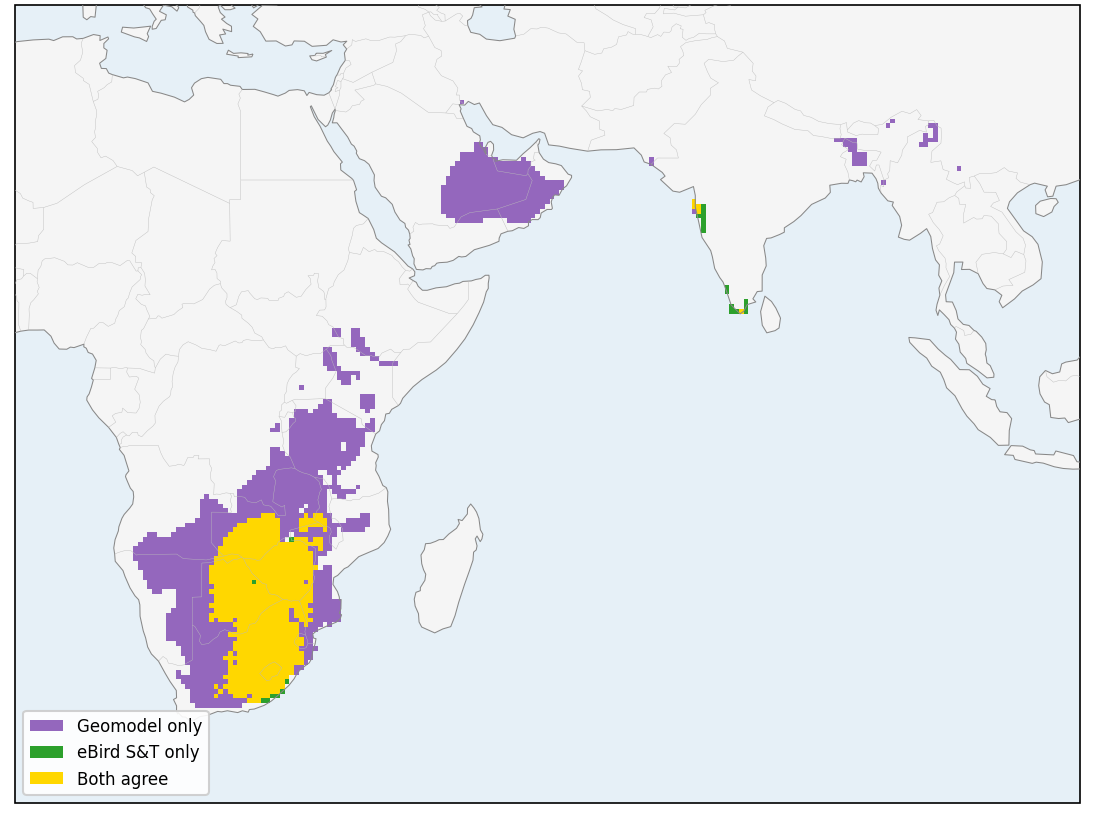
\includegraphics[width=\linewidth]{figures/ebirdst_amufal1_week1.png}
  \caption{Amur Falcon, week 1}
\end{subfigure}
\hfill
\begin{subfigure}[t]{0.48\linewidth}
  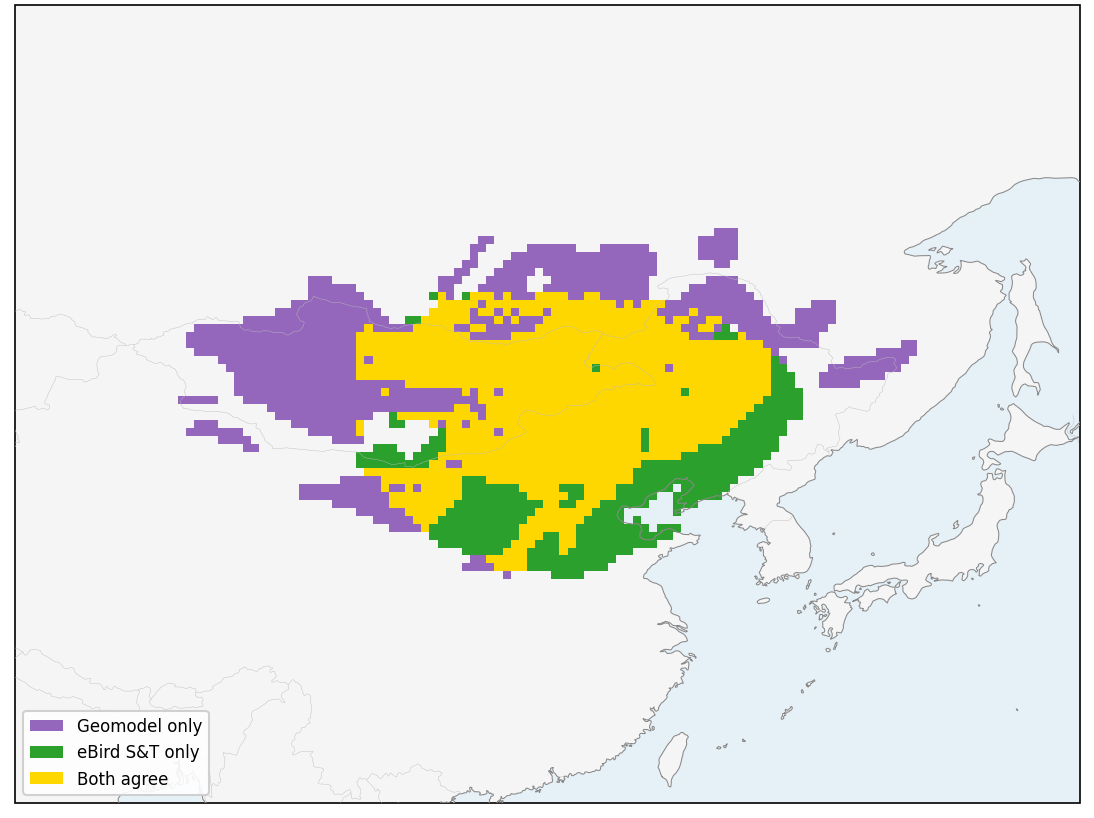
\includegraphics[width=\linewidth]{figures/ebirdst_amufal1_week26.png}
  \caption{Amur Falcon, week 26}
\end{subfigure}

\vspace{6pt}

\begin{subfigure}[t]{0.48\linewidth}
  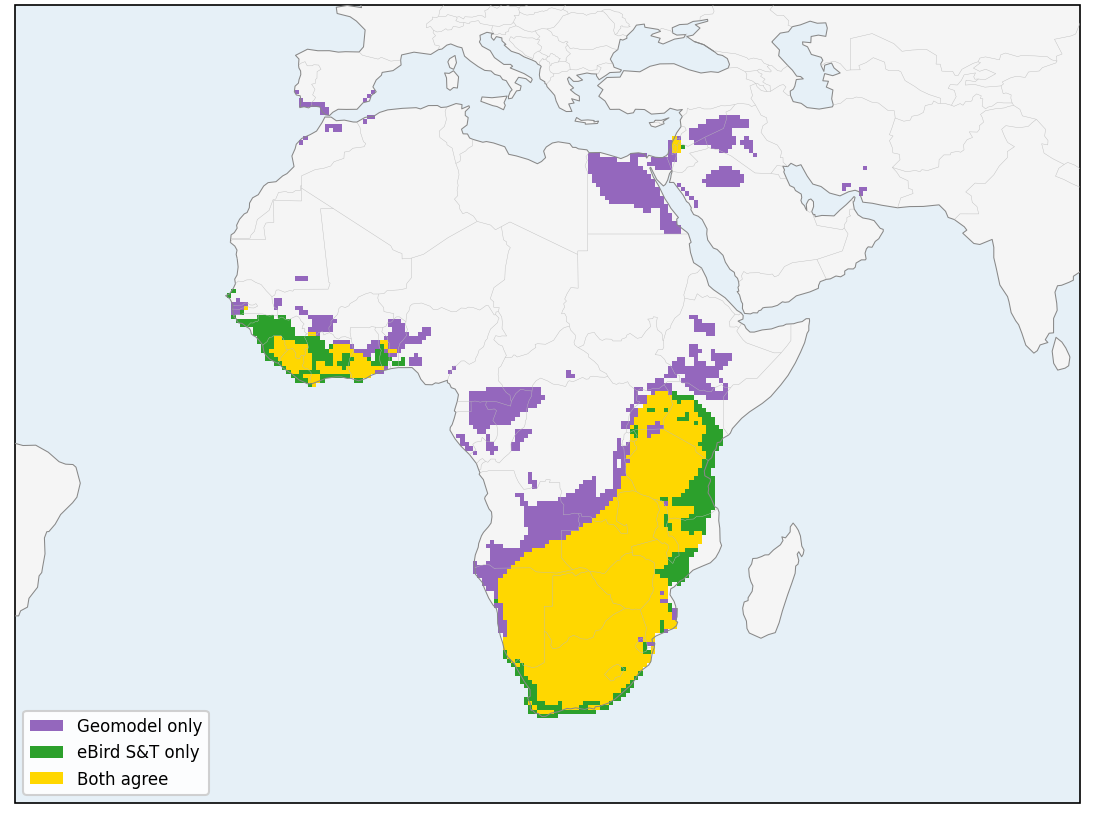
\includegraphics[width=\linewidth]{figures/ebirdst_comswi_week1.png}
  \caption{Common Swift, week 1}
\end{subfigure}
\hfill
\begin{subfigure}[t]{0.48\linewidth}
  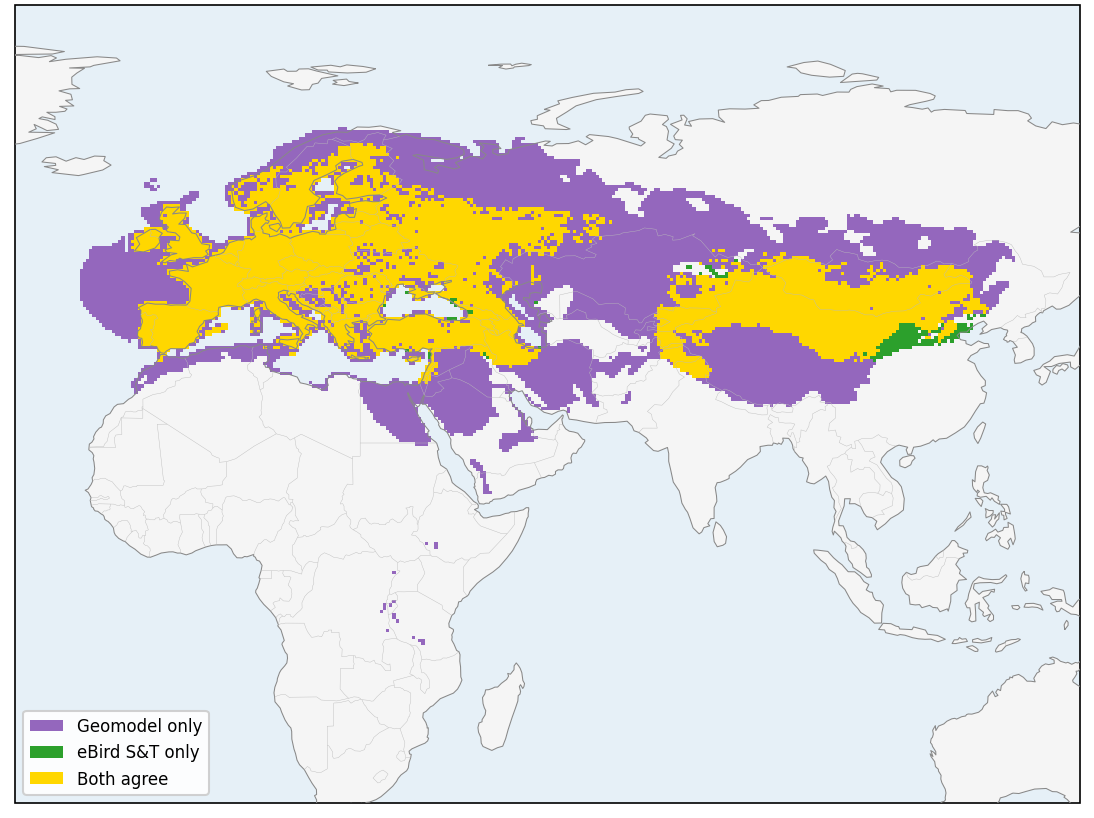
\includegraphics[width=\linewidth]{figures/ebirdst_comswi_week26.png}
  \caption{Common Swift, week 26}
\end{subfigure}

\vspace{6pt}

\begin{subfigure}[t]{0.48\linewidth}
  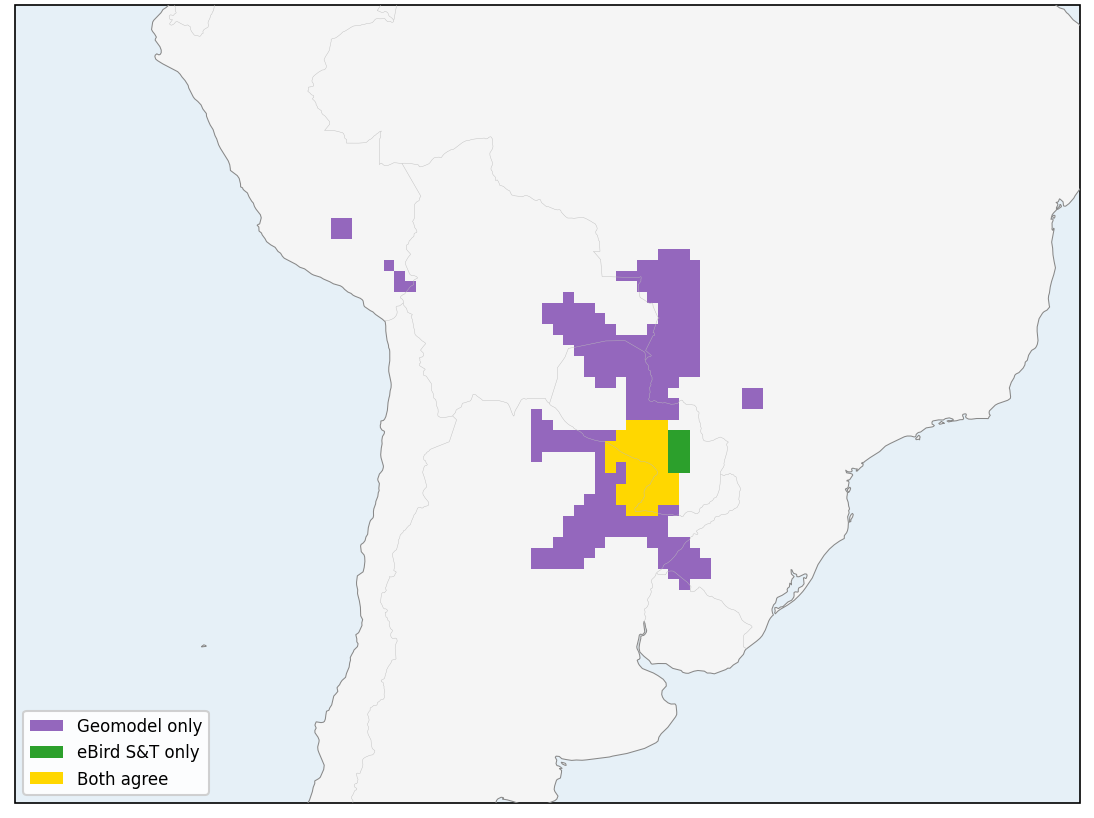
\includegraphics[width=\linewidth]{figures/ebirdst_boboli_week1.png}
  \caption{Bobolink, week 1}
\end{subfigure}
\hfill
\begin{subfigure}[t]{0.48\linewidth}
  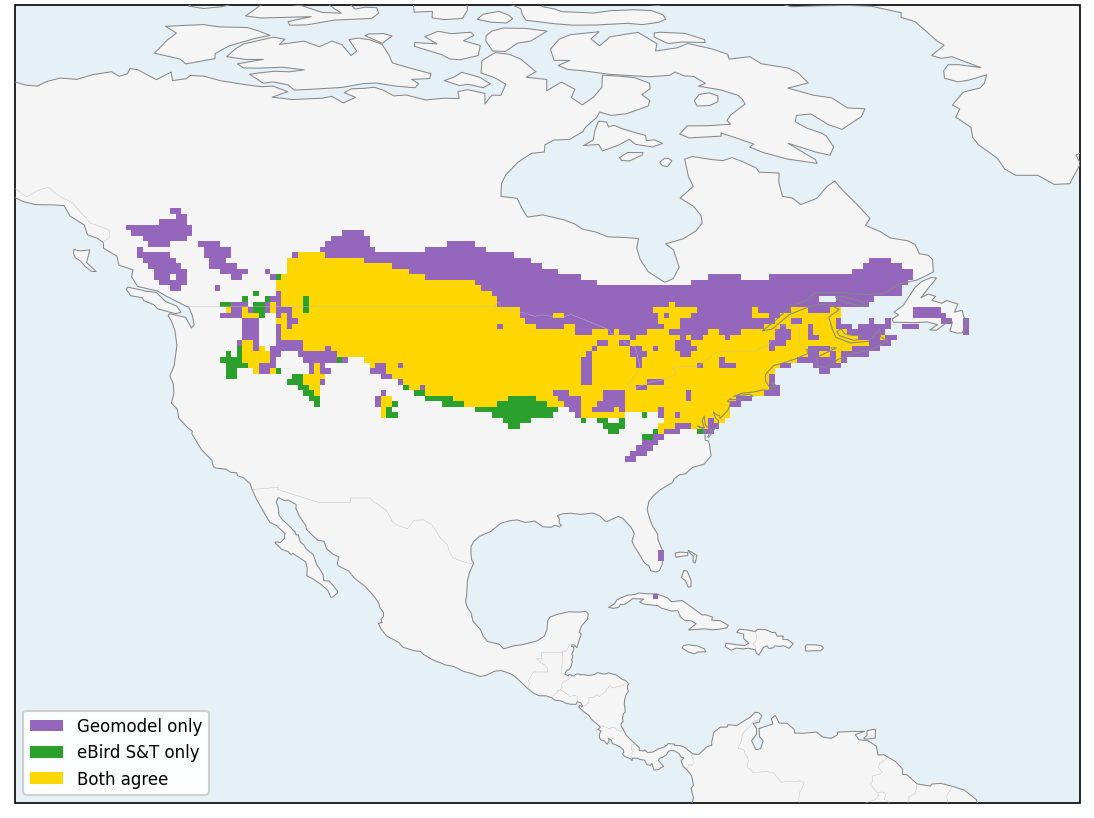
\includegraphics[width=\linewidth]{figures/ebirdst_boboli_week26.png}
  \caption{Bobolink, week 26}
\end{subfigure}
\caption{Range overlap with eBird Status and Trends for three long-distance migrants in
January (left) and July (right). Purple marks cells the geomodel predicts but S\&T does
not, green marks cells S\&T reports but the geomodel misses, and yellow marks agreement.
Each species reverses hemispheres between the two weeks, and the model tracks that
reversal from coordinates and week alone: Amur Falcon moves from southern Africa to
central Asia, Common Swift from sub-Saharan Africa to the Palearctic, and Bobolink from
South to North America. The characteristic disagreement is a purple fringe at range margins. Part of it is genuine
over-prediction; part is S\&T declining to assert presence where its data is thin, which the
comparison cannot separate (Section~\ref{sec:6-5-caveats}).
Metrics for all ten comparison species are in Table~\ref{tab:3}.}
\label{fig:6}
\end{figure}


\begin{figure}[p]
\centering
%% Two residents and one medium-distance migrant, each at both comparison weeks.
\begin{subfigure}[t]{0.48\linewidth}
  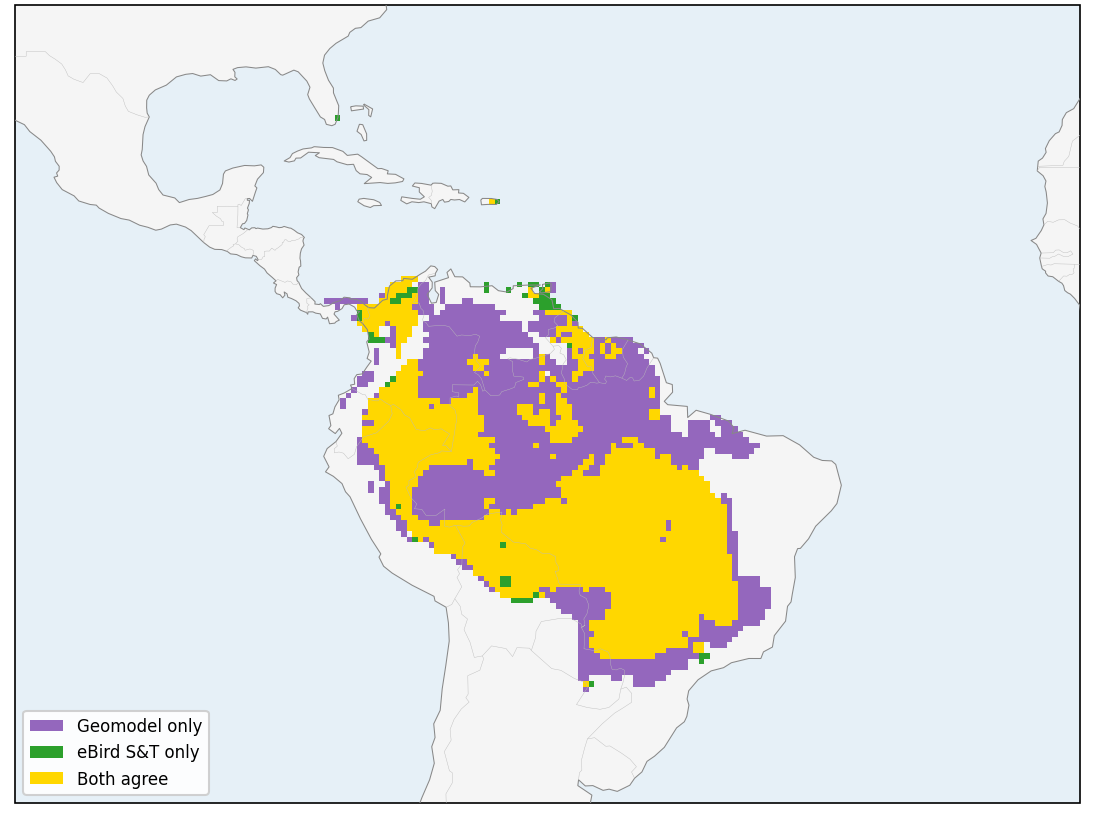
\includegraphics[width=\linewidth]{figures/ebirdst_baymac_week1.png}
  \caption{Blue-and-yellow Macaw, week 1}
\end{subfigure}
\hfill
\begin{subfigure}[t]{0.48\linewidth}
  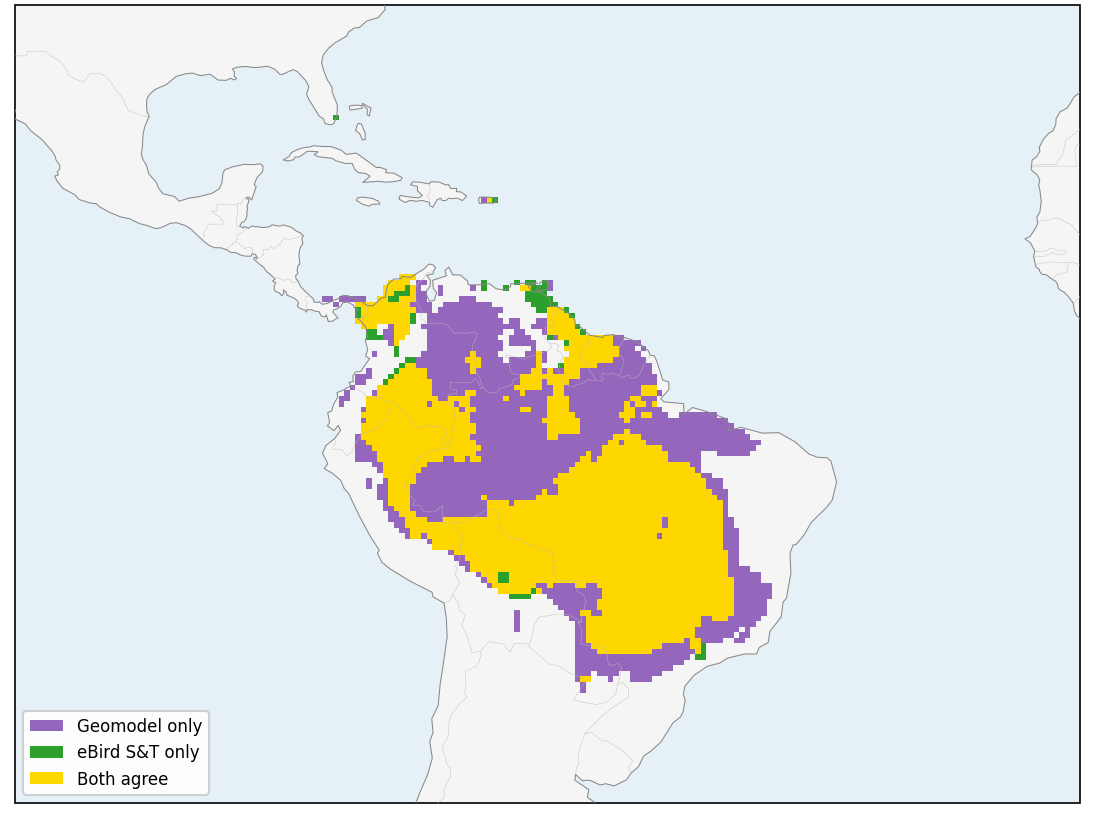
\includegraphics[width=\linewidth]{figures/ebirdst_baymac_week26.png}
  \caption{Blue-and-yellow Macaw, week 26}
\end{subfigure}

\vspace{6pt}

\begin{subfigure}[t]{0.48\linewidth}
  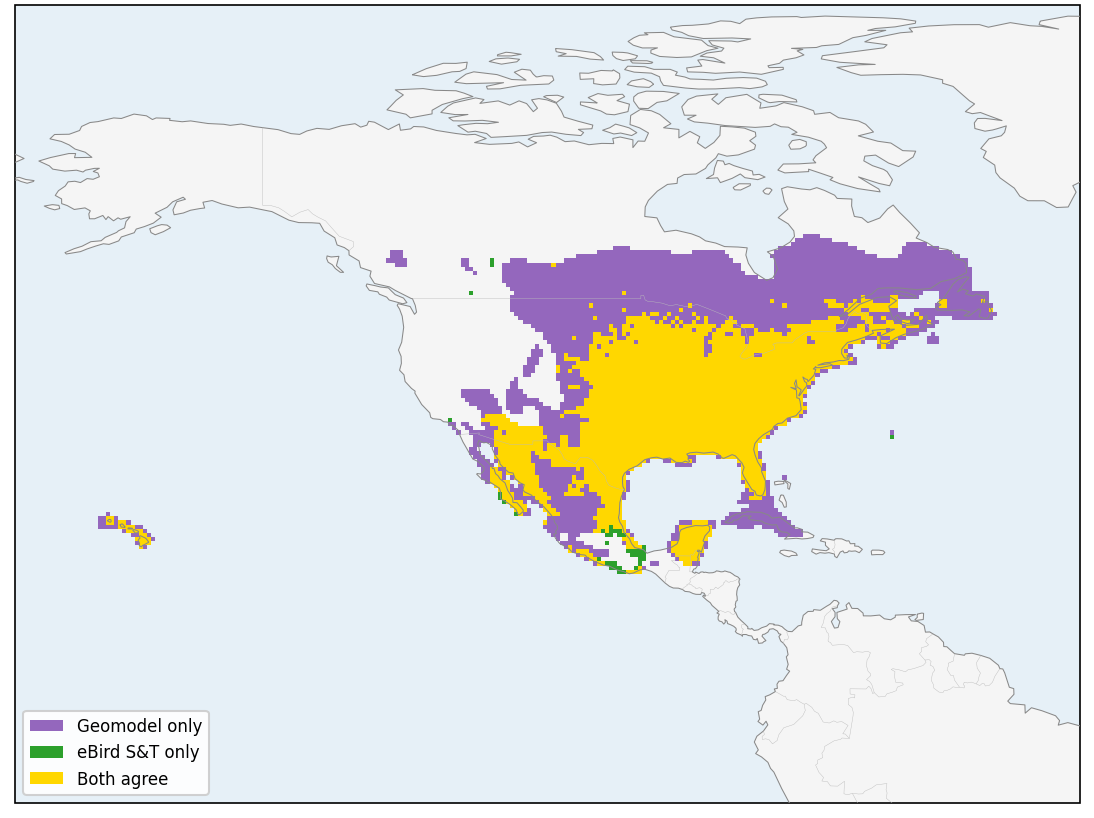
\includegraphics[width=\linewidth]{figures/ebirdst_norcar_week1.png}
  \caption{Northern Cardinal, week 1}
\end{subfigure}
\hfill
\begin{subfigure}[t]{0.48\linewidth}
  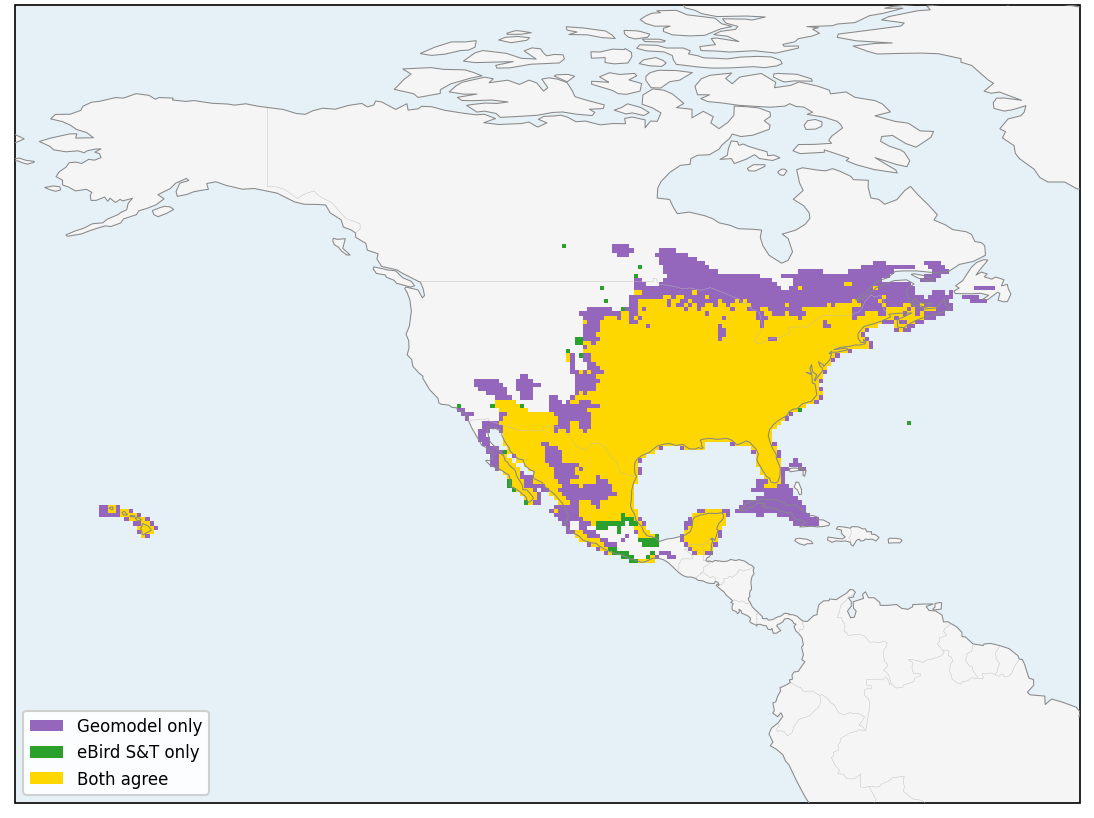
\includegraphics[width=\linewidth]{figures/ebirdst_norcar_week26.png}
  \caption{Northern Cardinal, week 26}
\end{subfigure}

\vspace{6pt}

\begin{subfigure}[t]{0.48\linewidth}
  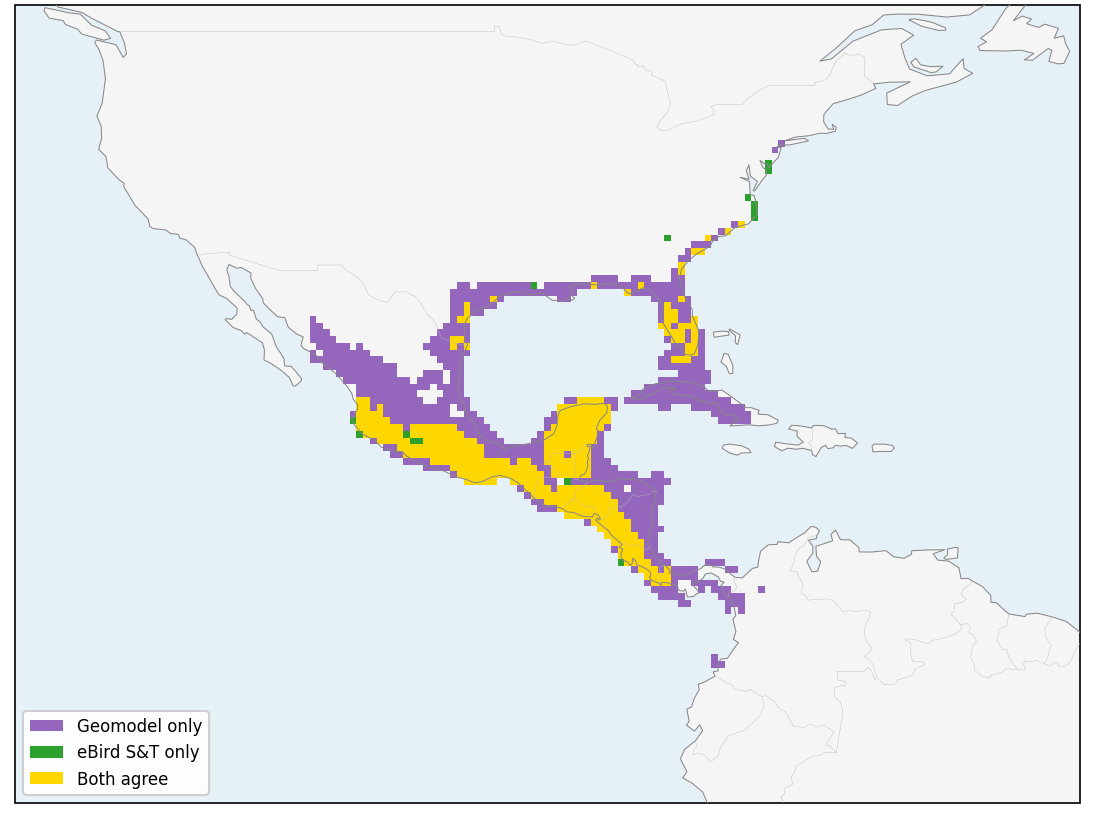
\includegraphics[width=\linewidth]{figures/ebirdst_rthhum_week1.png}
  \caption{Ruby-throated Hummingbird, week 1}
\end{subfigure}
\hfill
\begin{subfigure}[t]{0.48\linewidth}
  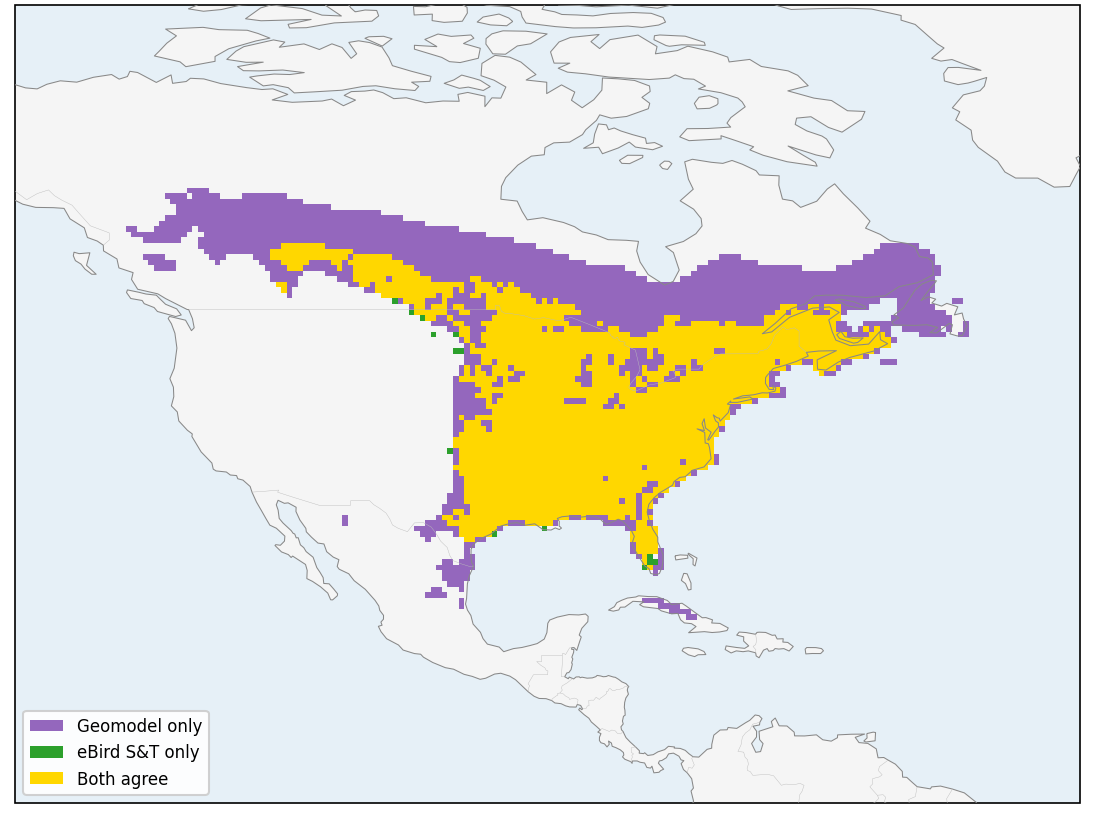
\includegraphics[width=\linewidth]{figures/ebirdst_rthhum_week26.png}
  \caption{Ruby-throated Hummingbird, week 26}
\end{subfigure}
\caption{Range overlap for two residents and one medium-distance migrant, in January
(left) and July (right); colors as in Figure~\ref{fig:6}. The two residents are nearly
identical across seasons (Blue-and-yellow Macaw Jaccard 0.690 versus 0.720; Northern
Cardinal 0.590 versus 0.684), confirming that the weekly conditioning does not introduce
spurious seasonality where none exists. Ruby-throated Hummingbird shows the study's
typical winter failure mode: the January panel over-predicts across Central America,
where S\&T concentrates the species into a narrower wintering band, which is what drives
its low January Jaccard of 0.407.}
\label{fig:7}
\end{figure}

\subsection{Caveats}
\label{sec:6-5-caveats}

Several factors qualify this comparison. Both models train on eBird data, so agreement partly reflects a shared data source rather than independent validation; disagreement is therefore more informative, revealing where the coordinate-only approach diverges from S\&T's covariate-driven methodology. The binarization threshold (0.15) is a round, practically convenient value within 0.3\% of the mean-F1 optimum (0.167); it simulates realistic usage but may not be optimal for individual species --- AUC, being threshold-free, is the most robust metric. S\&T maps have NaN outside modeled regions, so species with broad ranges are evaluated only on the subset where S\&T has data --- and that masking is not neutral for our metrics. S\&T withholds predictions precisely where observations are sparse, which is where a coordinate-only model is most likely to extrapolate and least likely to be checkable. Within the mask the same conservatism operates more subtly, since cells with thin sampling are reported as absent rather than uncertain. Both effects push measured precision down without evidence that the geomodel is wrong, so the precision figures in Table~\ref{tab:3} should be treated as a floor rather than an estimate. The 0.5\textdegree{} comparison grid (\textasciitilde{}55 km at the equator) smooths fine-scale range boundaries.


\section{Post-Filter Study on BirdNET App Submissions}
\label{sec:7-post-filter-study-on-birdnet-app-submiss}

Section~\ref{sec:6-comparison-with-ebird-status-and-trends} evaluates the geomodel as species distribution models are conventionally evaluated: by the fidelity of its probability surfaces to a reference range map. This is not the configuration in which the model is deployed. In production it is applied after the acoustic classifier and addresses a narrower question --- whether a species is plausible at a given location in a given week --- and its errors are asymmetric, since an over-inclusive candidate list is of little consequence whereas suppressing a species that was present is not recoverable. This section evaluates that deployment configuration directly, on recordings submitted through the BirdNET mobile app \citep{wood2022machine} rather than on reference maps. Selection and sampling details are given in Appendix~\ref{sec:F-post-filter-study-selection-and-sampling}.

The quantity measured is \emph{selectivity}: how much of the candidate list the filter removes, and at which ranks and confidence levels. Whether the underlying species identifications are correct is not measured, as these submissions carry no verified identifications and obtaining them would require expert review of 100,000 recordings. Selectivity is nonetheless the property that governs whether the filter can be deployed safely, since it determines how often the filter contradicts the classifier's primary prediction.

\subsection{Methodology}
\label{sec:7-1-methodology}

From the 39.6 M app submissions recorded in 2025 --- each a short recording with a location, a timestamp, and the on-device classifier's top detections \citep{wood2022machine} --- we retain those with a confident on-device detection (score > 0.5), no human vocalization among the ten reported classes, a duration of 2.5--3.5 s (so that a single centered 3 s window covers the recording), and valid coordinates and date, yielding 1,718,002 candidates. As this pool is 83.7\% European, we subsample it with an equal quota per occupied H3 resolution-2 cell (\textasciitilde{}86,000 km$^2$), rotating over cells and over devices within each cell and redistributing the quota of exhausted cells across the remainder. The result is \textbf{100,032 recordings across 1,216 cells}, with the European share reduced to 39.0\% and Asia, South America and Oceania each increasing five- to thirteen-fold (Figure~\ref{fig:8}).

Each recording's centered 3 s window is classified with the BirdNET+ V3.0 developer preview (\texttt{V3.0-preview3.1\_Global\_11K}, 11,560 classes, 32 kHz input; \citealp{lasseck2026birdnetv3}). For every top-3 prediction of class \emph{Aves} we query the geomodel at the recording's (latitude, longitude, week) and mark the prediction \textbf{rejected} if its occurrence probability falls below \textbf{$t = 0.15$} --- the same operating point used in Section~\ref{sec:6-comparison-with-ebird-status-and-trends} Classes are matched between the two label sets by scientific name; 99.37\% of bird predictions have a geomodel counterpart, and the remainder are excluded rather than counted as rejections.

Results are reported against two axes: the prediction's \emph{rank} --- rank 1 being the identification presented to the user, ranks 2 and 3 the alternatives the classifier scored lower --- and its \emph{confidence}. Jointly these characterize where in the candidate list the filter acts.

\begin{figure}[htbp]
\centering
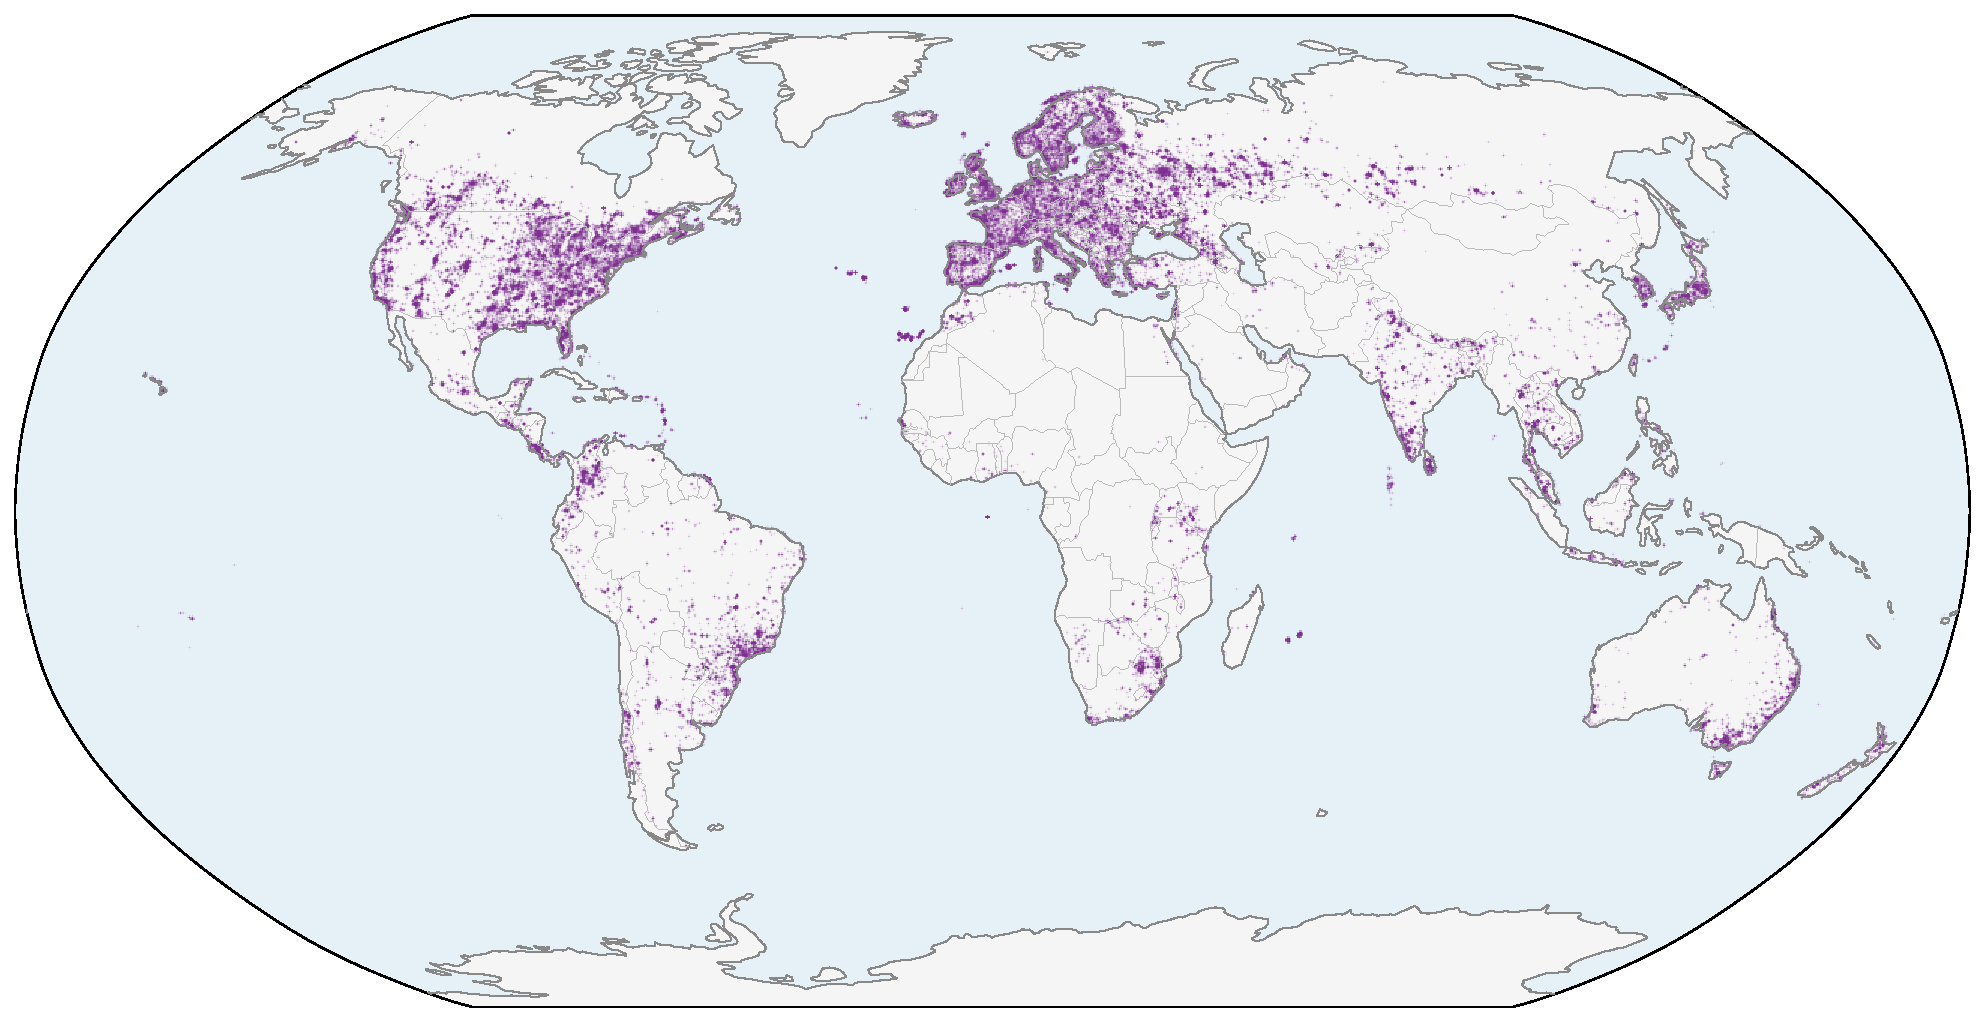
\includegraphics[width=\linewidth]{figures/filter_study_sample_map.pdf}
\caption{The study set: 100,032 BirdNET app submissions from 2025, drawn with an equal quota per occupied H3 resolution-2 cell. Balancing cuts the European share of the pool from 83.7\% to 39.0\% and multiplies the Asian, South American, and Oceanian shares five- to thirteen-fold; what remains visible is the residual density within regions, since the quota equalises cells rather than area.}
\label{fig:8}
\end{figure}

\subsection{Results}
\label{sec:7-2-results}

At $t = 0.15$ the geomodel rejects 58,396 of 296,251 bird predictions (19.7\%). The aggregate rate is of limited interest on its own; the informative result is its distribution over prediction rank and classifier confidence.


\begin{table}[!ht]
\centering
\caption{Geomodel post-filter on the top-3 bird predictions of the study set at threshold 0.15; confidence buckets pool all three ranks. The contrast between the rank rows and the confidence rows is the result: the filter removes a quarter of the runner-up candidates and one in fifty of the predictions the classifier is confident about.}
\label{tab:4}
\small
\begin{tabular}{lrrr}
\toprule
Prediction group & Predictions & Rejected & Rejection rate \\
\midrule
Rank 1 & 99,764 & 4,769 & \textbf{4.8\%} \\
Rank 2 & 97,941 & 25,192 & 25.7\% \\
Rank 3 & 98,546 & 28,435 & 28.9\% \\
Confidence 0.90--1.00 & 50,324 & 1,064 & \textbf{2.1\%} \\
Confidence 0.75--0.90 & 37,093 & 1,187 & 3.2\% \\
Confidence 0.25--0.50 & 17,993 & 3,214 & 17.9\% \\
Confidence 0.05--0.10 & 21,604 & 7,985 & \textbf{37.0\%} \\
Rank-2/3 below confidence 0.05 & 127,622 & 36,685 & 28.8\% \\
\textbf{All bird predictions} & \textbf{296,251} & \textbf{58,396} & \textbf{19.7\%} \\
\bottomrule
\end{tabular}
\end{table}

The filter removes approximately a quarter of the second- and third-ranked candidates but only 4.8\% of top-1 predictions and 2.1\% of predictions above 0.90 confidence. Above a confidence of 0.25 the rejection rate declines monotonically and steeply (Figure~\ref{fig:filter-rate}). Per recording, 2.38 of 2.96 scored bird candidates survive; 41.1\% of recordings lose at least one candidate and 2.0\% lose all three, the latter being the case in which a post-filter would return an empty candidate list.

The threshold itself is not a sensitive parameter (Figure~\ref{fig:filter-sweep}). Between $t = 0.02$ and $t = 0.20$ the rank-1 rejection rate moves only from 2.5\% to 5.8\% while rank-2/3 rejections stay above 20\% throughout, because the geomodel's scores for top-1 predictions are strongly bimodal (median 0.843). Only beyond $t = 0.3$ does the cost to top-1 predictions rise sharply (16.3\% at $t = 0.5$).

\begin{figure}[htbp]
\centering
\begin{subfigure}[t]{0.49\linewidth}
  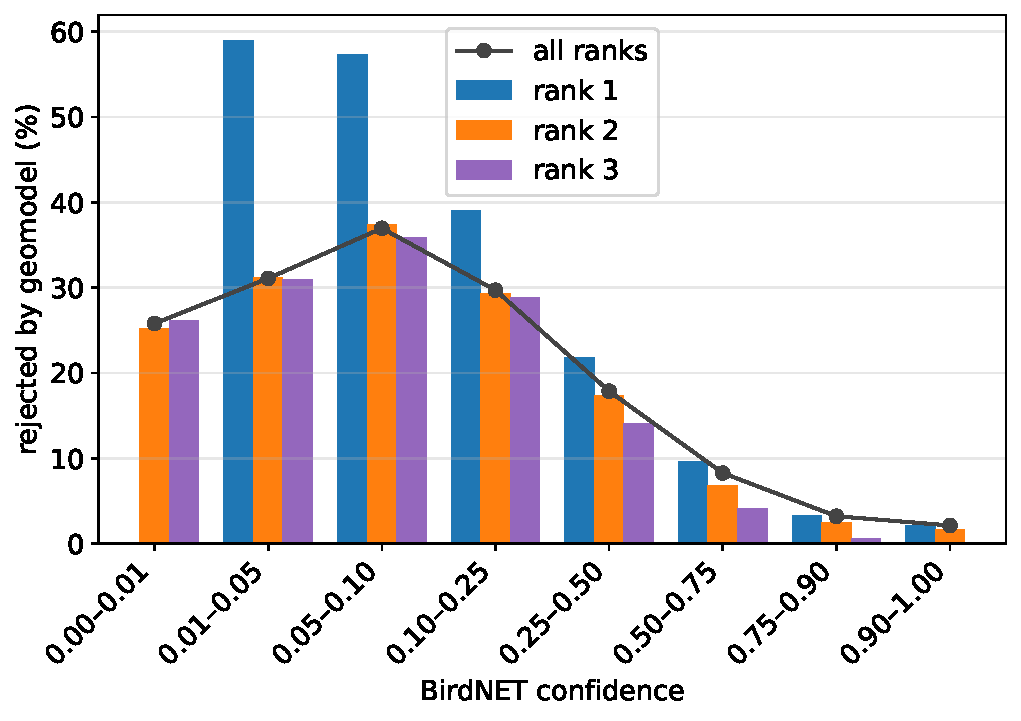
\includegraphics[width=\linewidth]{figures/filter_study_rejection_by_confidence.pdf}
  \caption{Rejection rate}
  \label{fig:filter-rate}
\end{subfigure}
\hfill
\begin{subfigure}[t]{0.49\linewidth}
  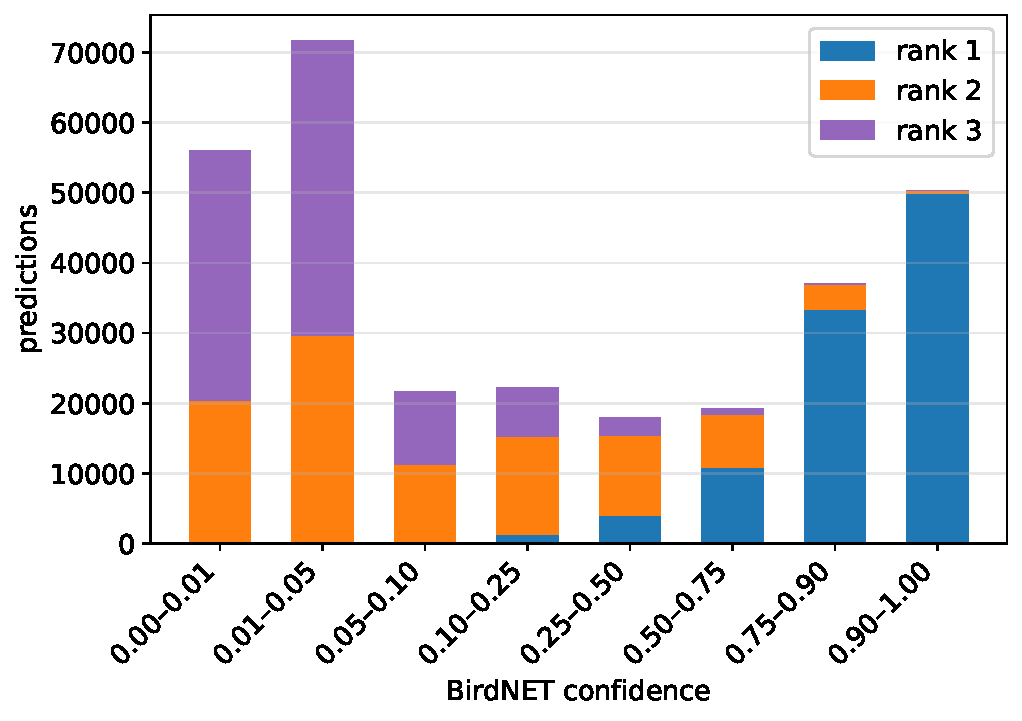
\includegraphics[width=\linewidth]{figures/filter_study_bucket_volume.pdf}
  \caption{Prediction volume}
  \label{fig:filter-volume}
\end{subfigure}

\vspace{8pt}

\begin{subfigure}[t]{0.49\linewidth}
  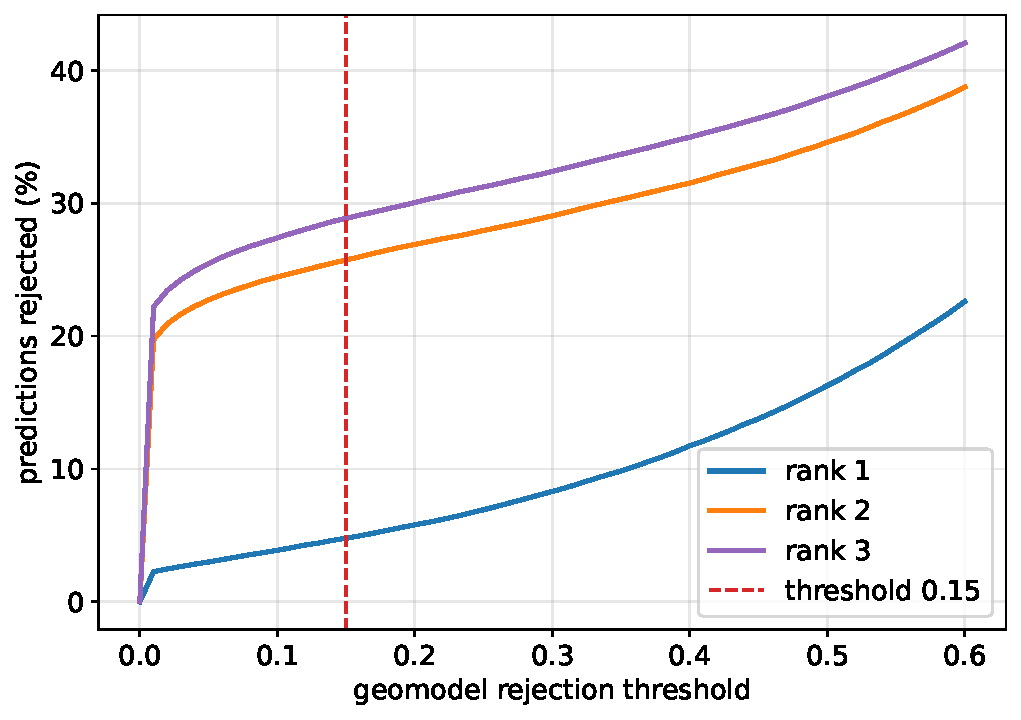
\includegraphics[width=\linewidth]{figures/filter_study_threshold_sweep.pdf}
  \caption{Threshold sensitivity}
  \label{fig:filter-sweep}
\end{subfigure}
\hfill
\begin{subfigure}[t]{0.49\linewidth}
  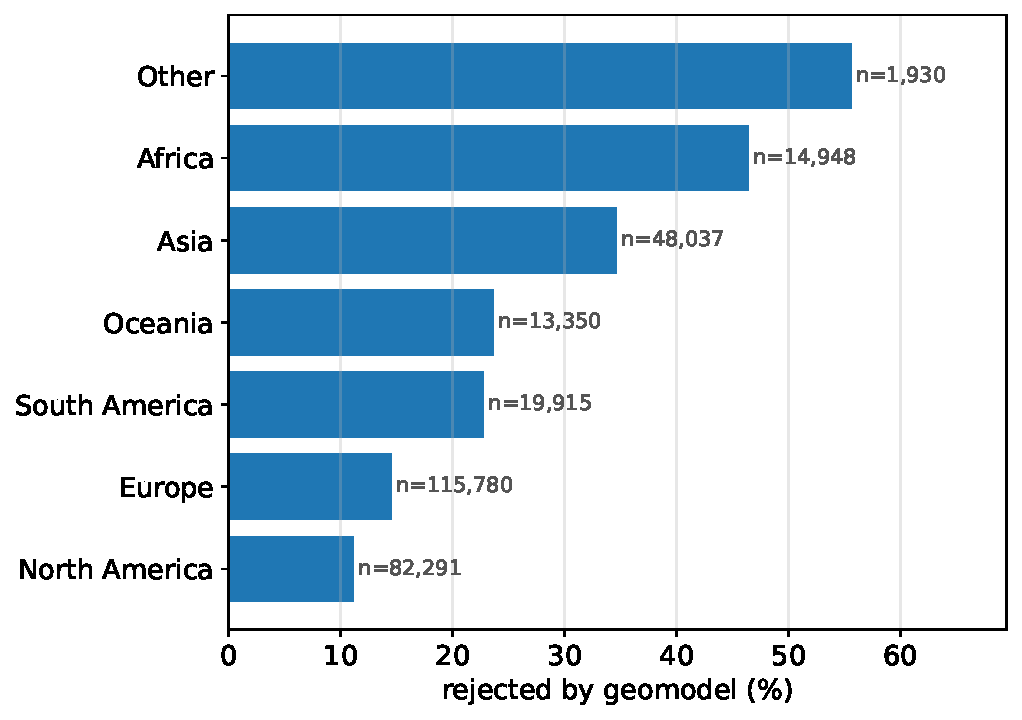
\includegraphics[width=\linewidth]{figures/filter_study_rejection_by_region.pdf}
  \caption{Rejection rate by region}
  \label{fig:filter-region}
\end{subfigure}
\caption{Geomodel post-filter applied to the top-3 bird predictions of the study set at
threshold $t = 0.15$. (a) Rejection rate per confidence bucket, split by prediction rank,
with the pooled rate as a dark line; bars are drawn where at least 25 predictions fall in
the bucket. The rate falls monotonically above a confidence of 0.25 and reaches 2.1\% in
the top bucket, so the filter and the classifier rarely disagree where the classifier is
sure. (b) How many predictions each bucket holds: the rejections concentrate in the
low-confidence tail rather than among the identifications a user is shown. (c) Varying
the threshold between 0.02 and 0.20 moves the rank-1 rejection rate by only three
percentage points, because the geomodel's scores for top-1 predictions are strongly
bimodal; the dashed line marks the operating point inherited from Section~\ref{sec:6-comparison-with-ebird-status-and-trends}. (d) The same
filter intervenes three to four times more often in Africa and Asia than in North
America --- the study's main caveat, discussed in Section~\ref{sec:7-4-caveats}.}
\label{fig:9}
\end{figure}

The species removed most frequently are those a global classifier is expected to over-predict outside their ranges: Northern Cardinal (2,974 rejections, almost all as low-scoring rank-2/3 candidates), Common Blackbird (1,007, predominantly in Asia and Africa), American Robin (736, predominantly in Europe and Asia) and Red-winged Blackbird (489). The 839 North American cardinal rejections are consistent with the species' range rather than contradicting it: 80.2\% lie west of 100\textdegree{} W or north of 50\textdegree{} N.

\subsection{Interpretation}
\label{sec:7-3-interpretation}

The same probability surfaces that yield a mean Jaccard of 0.632 against eBird S\&T leave 97.9\% of high-confidence predictions untouched while removing roughly a quarter of the low-ranked alternatives. The two evaluations measure different properties of a single model: fidelity to a reference range map in Section~\ref{sec:6-comparison-with-ebird-status-and-trends}, and selectivity within a candidate list here. Only the second corresponds to the deployed task, and it provides the empirical basis for the design philosophy set out in Section~\ref{sec:8-1-design-philosophy-a-filter-not-a-full-sd}.

The over-inclusiveness reported in Section~\ref{sec:6-comparison-with-ebird-status-and-trends} --- recall 0.910 against precision 0.683 --- is the property that makes this possible. It keeps top-1 rejection at 4.8\% rather than at a level at which the filter would routinely contradict the classifier, and it implies that the model's known over-extension into coastal waters renders the filter more permissive near coasts rather than less. For range mapping these are deficiencies; for filtering they are the preferable direction of error.

\subsection{Caveats}
\label{sec:7-4-caveats}

First, rejection rates vary strongly by region (Figure~\ref{fig:filter-region}): 11.2\% in North America and 14.5\% in Europe against 34.6\% in Asia and 46.4\% in Africa. Two mechanisms push in the same direction and this design cannot separate them --- the acoustic classifier makes more out-of-range errors where its training data is sparse, and the geomodel's occurrence surfaces are least reliable in exactly those regions. The regional figures should therefore not be read as a measurement of classifier error alone.

Second, the study measures selectivity, not correctness. Without verified identifications, the 4.8\% of rejected top-1 predictions cannot be separated into correctly caught out-of-range errors and wrongly suppressed rarities. Vagrants and range-edge records are by construction concentrated in the rejected set, and they are the one population a filter of this kind can harm.

Third, the selection criteria --- a confident on-device detection and a 2.5--3.5 s duration --- favor short, clean recordings, so rejection rates on the unfiltered submission stream would likely be higher than those reported here.


\section{Discussion}
\label{sec:8-discussion}

\subsection{Design Philosophy: A Filter, Not a Full SDM}
\label{sec:8-1-design-philosophy-a-filter-not-a-full-sd}

The key distinction is between what our model is \emph{meant} to do and what a classical species distribution model attempts. BirdNET Geomodel is not meant to replace curated range maps, effort-corrected abundance surfaces, or independently validated SDMs. Its role is narrower and more pragmatic: given a geographic location and a week of year, it must quickly narrow a vocabulary of over 10,000 species down to the ecologically plausible subset, so that an audio classifier does not waste probability mass on species that could not realistically be present. A geographically implausible detection --- a Common Myna flagged in Minnesota, or a European Bee-eater in Brazil --- is simply noise; the geomodel exists to suppress it.

This framing has direct consequences for how we evaluate success. A filtering model needs to be \emph{good enough}: it should reliably include species that are present (high recall) and not grossly over-include species that are absent (reasonable precision). It does not need ecological accuracy at the level of a published range map, nor does it need to distinguish fine-scale habitat within a 26 km H3 cell. The GeoScore reflects this: its components weight discrimination (mAP 0.20, F1 0.20) and spatial fairness (density ratio 0.20) heavily, with calibration (list ratio 0.15) and robustness to survey effort (watchlist AP 0.10, pred--density correlation 0.05) as supporting objectives. The eBird S\&T comparison (Section~\ref{sec:6-comparison-with-ebird-status-and-trends}) --- mean AUC 0.975, mean F1 0.764 at threshold 0.15 --- confirms that the model meets this bar: it gets the gross range geometry right across guilds, migration strategies, and hemispheres, which is precisely what a filter needs to do.

The post-filter study of Section~\ref{sec:7-post-filter-study-on-birdnet-app-submiss} provides direct evidence for this framing. On 100,032 globally balanced app submissions the model rejects 25.7\% and 28.9\% of the classifier's second- and third-ranked candidates, but only 4.8\% of its top-1 predictions and 2.1\% of predictions above 0.90 confidence. The surfaces that appear unremarkable when scored as range maps (mean Jaccard 0.632 against S\&T) therefore act, in the deployed configuration, as a filter that removes the low-confidence portion of the candidate list while seldom contradicting a confident prediction. These are two evaluations of one model rather than two models: a variant tuned to maximize Jaccard against a reference range map would plausibly be a \emph{worse} filter, since precision gained at range margins is paid for in recall precisely where vagrants and range-edge records occur.

Several design choices follow directly from this philosophy. At approximately 7 MB in FP16 (scale 0.75), the model must run on the devices where BirdNET Analyzer, the BirdNET mobile app, Haikubox, and BirdWeather are deployed --- staying well under the <10 MB mobile budget. A heavier model that marginally improves watchlist AP on island endemics is not a useful trade. No environmental covariates are needed at inference: querying elevation databases or land-cover APIs at detection time would be impractical in the field. And the 48-week temporal resolution --- sufficient to capture migration, breeding phenology, and winter range contraction --- is coarser than the 52-week S\&T calendar but fine enough that no species shifts from present to absent within a single model-week under realistic conditions.

\subsection{The Primacy of Label Propagation}
\label{sec:8-2-the-primacy-of-label-propagation}

Label propagation accounts for two of the three largest GeoScore gains in the ablation: enabling it (+31\%, Stage C) and optimizing its parameters (+13\%, Stage H). Together, these represent a 48\% cumulative improvement over the pre-propagation baseline. The mechanism can be understood as a form of spatial data augmentation on the target labels: by copying species lists from observed cells to environmentally similar unobserved cells, it forces the model to learn distributions in regions where it would otherwise receive no training signal. The result is a structural redistribution of performance --- sparse-region mAP jumps from 0.28 to 0.87, while the density ratio converges from 1.22 to 0.973 --- because the model has been explicitly exposed to the assemblages it needs to filter in under-surveyed parts of the world.

The ecological constraints introduced in Stage H are essential. Without them, the optimizer discovers that GeoScore rewards aggressive propagation up to a point and pushes parameters toward implausible extremes (radii exceeding 5,000 km). The environmental-distance gate and per-species range cap redirect optimization toward ecologically valid cells. The modest drop in watchlist AP (0.635 $\rightarrow$ 0.535) reflects the tension between filling global coverage gaps and preserving crisp boundaries for island endemics --- a tradeoff that is explicitly acceptable given the filter framing: a species endemic to a single island will simply not appear in most audio detections regardless of whether the model's confidence boundary is at 50 km or 200 km.

\subsection{Calibration, Scale, and Architectural Choices}
\label{sec:8-3-calibration-scale-and-architectural-choi}

\textbf{Loss function.} All four loss families achieve nearly identical species ranking (mAP 0.536--0.544), but calibration varies by orders of magnitude: BCE produces list ratios \textasciitilde{}6$\times$ at 10\%, while aggressive ASL inflates this to \textasciitilde{}979$\times$. Focal-style down-weighting encourages the model to assign high probability to all species once the easy negatives are suppressed, which is catastrophic for a filter. BCE with light label smoothing (0.05) avoids this failure mode and is the clear practical choice.

\textbf{Model scale.} Scaling from 0.5 to 2.0 improves GeoScore by 5.6\% in coordinate-only mode (0.408 $\rightarrow$ 0.431), split evenly between the two doublings --- a consistent but modest gain. Scale 2.0 wins the ablation, but at \textasciitilde{}47M parameters it is far outside the deployment budget, and scale 1.0 (7.2M parameters, \textasciitilde{}14 MB FP16) still exceeds the <10 MB mobile target. Scale 0.75 (3.8M parameters, \textasciitilde{}7 MB FP16) is the production operating point: it fits well under the mobile budget while retaining most of the capacity benefit of scale 1.0.

\textbf{Environmental auxiliary task.} The auxiliary task provides no benefit to species prediction quality --- the model learns environmental gradients implicitly from species co-occurrence patterns. We retain it because it has negligible cost and its intermediate representations may serve downstream tasks (habitat classification, abundance transfer learning). The habitat head adds complexity with no metric improvement and is not recommended.

\subsection{Comparison with Existing Approaches}
\label{sec:8-4-comparison-with-existing-approaches}

Our model inherits the coordinate-only paradigm of SINR \citep{cole2023spatial} but adds weekly temporal resolution via FiLM conditioning and multi-harmonic encoding for finer spatial boundaries, producing 48 distinct occurrence surfaces per species rather than a single static range map. The eBird Status and Trends products \citep{fink2024ebird} also operate at weekly resolution but model each species independently with effort covariates and adaptive ensembles --- an approach that achieves greater ecological precision at the cost of being unsuitable for on-device deployment across over 10,000 species. GeoLifeCLEF benchmarks \citep{botella2025geolifeclef} evaluate multi-species occurrence at continental scale, and the finding by \citet{kellenberger2026performance} that DL models match but do not surpass classical SDMs --- and underperform for threatened species --- is a useful caution: our watchlist component (10\% GeoScore weight) and density-stratified evaluation are designed to surface precisely these failure modes, even if fully closing them is outside the scope of a filtering model.

\subsection{Operating the Filter in Practice}
\label{sec:8-5-operating-the-filter-in-practice}

Three operational conclusions follow from Section~\ref{sec:7-post-filter-study-on-birdnet-app-submiss}

\textbf{Threshold selection is not critical.} Anywhere between $t = 0.02$ and $t = 0.20$, the rank-1 rejection rate moves only from 2.5\% to 5.8\% while rank-2/3 rejections stay above 20\%. The geomodel's scores for top-1 predictions are strongly bimodal, so the consequential decision is whether to filter at all rather than where precisely to place the boundary. The value $t = 0.15$, inherited from the S\&T comparison, is a defensible default rather than a tuned one, and the submission data provide no evidence for revising it.

\textbf{The filter acts predominantly where the classifier is uncertain.} Rejection rates fall monotonically above a classifier confidence of 0.25, reaching 2.1\% in the top bucket; above 0.75 the filter is close to inactive. A confidence-gated variant that applies the geomodel only to the contested middle of the score range would therefore forfeit few rejections while eliminating most of the residual risk to confident predictions. Such a configuration is preferable wherever false suppression is more costly than a spurious candidate, and it is the most direct extension of this study.

\textbf{The intervention rate is strongly region-dependent.} Rejection rates in Africa (46.4\%) and Asia (34.6\%) are three to four times those in North America (11.2\%). Whether this reflects more classifier errors or weaker geomodel surfaces in under-sampled regions cannot be resolved with the available data; under either explanation, a globally uniform threshold causes the filter to intervene most strongly where both models are least reliable, which is the opposite of what a risk-averse configuration would do. Region-aware thresholds, or thresholds conditioned on local propagation quality, merit investigation before the filter is relied upon for automated data products in these regions. The mitigation available without further work is the confidence gate described above, which restricts intervention to predictions the classifier itself scores as uncertain.

\subsection{Limitations}
\label{sec:8-6-limitations}

Several factors constrain interpretation. Our data is presence-only: absences reflect non-detection, not verified absence. Label propagation fills gaps but produces approximations, not ground truth. The prediction--density correlation remains high (\textasciitilde{}0.90 pred--density r), indicating that the model still predicts richer communities in heavily surveyed areas; the near-optimal density ratio shows that this bias is balanced across quartiles, but the absolute coupling to observer effort has not been eliminated. The static nature of the model --- a single average over 2023 eBird observations --- means it cannot track real-time range shifts, invasive species spread, or year-to-year population change. The S\&T comparison (Section~\ref{sec:6-comparison-with-ebird-status-and-trends}) is not independent: both systems derive from eBird checklists, so agreement partly reflects shared training data. Validation against expert-curated range polygons (e.g., BirdLife International) would provide a truly independent spatial accuracy assessment, and would also resolve the asymmetry noted in Section~\ref{sec:6-5-caveats}: because S\&T withholds predictions where data is sparse, our measured precision against it is a lower bound rather than an estimate, and the cells where the two systems disagree most are precisely the ones neither can currently adjudicate. The post-filter study (Section~\ref{sec:7-post-filter-study-on-birdnet-app-submiss}) shares this weakness in a different form --- it lacks verified identifications altogether, so the small fraction of rejected top-1 predictions cannot be separated into correctly caught out-of-range errors and wrongly suppressed rarities. Vagrants and range-edge records are by construction concentrated in the rejected set, which is the one population the filter can harm and the one this evaluation cannot see. A labeled follow-up using the app's explicit user-confirmation field would convert that rejection rate into a genuine false-suppression rate.


\section{Conclusion}
\label{sec:9-conclusion}

We presented BirdNET Geomodel, a multi-task neural network that predicts weekly occurrence probabilities for over 10,000 species from raw geographic coordinates and week of year alone --- no environmental covariates at inference. The model compresses global spatiotemporal species distributions into approximately 7 MB (FP16), replacing hundreds of megabytes of raw observation data and enabling real-time species filtering on mobile phones and embedded acoustic sensors.

A staged ablation study comprising 46 grid-search experiments and 60 Bayesian optimization trials yields three principal findings. First, label propagation --- imputing species lists from well-observed cells to environmentally similar unobserved ones --- is by far the most impactful design choice, improving GeoScore by 31\% and increasing sparse-region mAP from 0.28 to 0.87. Second, loss function choice affects probability calibration far more than species ranking: all four loss families achieve similar mAP, but calibration varies by two orders of magnitude, making BCE with light label smoothing the clear default for filtering applications. Third, the model implicitly learns environmental gradients from species co-occurrence; explicit environmental auxiliary tasks add no measurable benefit to species prediction, though they produce useful embeddings for downstream applications at negligible cost.

Comparison with eBird Status and Trends confirms that the model produces ecologically plausible range geometry (mean AUC 0.975, mean F1 0.764 at threshold 0.15 across 10 species at two contrasting weeks), correctly capturing seasonal migrations despite using no environmental inputs. The main failure mode --- over-prediction in data-sparse wintering grounds --- is a desirable property for the intended filtering use case: an over-inclusive filter is far less harmful than a filter that silences species that are actually present.

A study of 100,032 globally balanced BirdNET app submissions from 2025 confirms this in deployment. Applied as a post-filter to the acoustic classifier's top-3 predictions, the geomodel rejects 25.7\% and 28.9\% of second- and third-ranked candidates but only 4.8\% of top-1 predictions and 2.1\% of predictions above 0.90 confidence, removing the low-confidence portion of the candidate list while seldom contradicting a confident prediction. The species it removes most often --- Northern Cardinal in Asia and western North America, Common Blackbird in Africa --- are exactly the out-of-range confusions a global classifier is expected to make. Rejection rates are three to four times higher in Africa and Asia than in North America, a regional imbalance that argues for confidence-gated or region-aware thresholds before the filter is relied on for automated data products in under-surveyed regions.

Several directions warrant future investigation. The model is currently static; extending it to capture inter-annual range shifts from climate and land-use change would require multi-year temporal encoding and training data with year-level labels. Finer spatial resolution (H3 level 5 or 6) could improve predictions near range boundaries but would demand substantially more training data. Targeted enrichment of observation data in under-surveyed tropical and marine regions would directly benefit propagation quality. Finally, the environmental embeddings learned by the auxiliary task offer a starting point for abundance prediction and habitat classification without additional environmental inputs at inference --- a direction we plan to explore in future work.


\section{Acknowledgements}
\label{sec:acknowledgements}

Our work in the Cornell K. Lisa Yang Center for Conservation Bioacoustics at the Cornell Lab of Ornithology is made possible by the generosity of K. Lisa Yang to advance innovative conservation technologies to inspire and inform the conservation of wildlife and habitats.

The development of BirdNET is supported by the German Federal Ministry of Research, Technology and Space (FKZ 01|S22072), the German Federal Ministry for the Environment, Climate Action, Nature Conservation and Nuclear Safety (FKZ 67KI31040E), the German Federal Ministry of Economic Affairs and Energy (FKZ 16KN095550), the Deutsche Bundesstiftung Umwelt (project 39263/01), and the European Social Fund.

Species occurrence data were obtained from the Global Biodiversity Information Facility (GBIF; \url{https://www.gbif.org}). Two separate downloads were used in this work:

\begin{enumerate}
  \item \textbf{Ablation experiments.} eBird, iNaturalist, and observation.org records downloaded
on 03 March 2026 (GBIF.org, 2026a; \url{https://doi.org/10.15468/dl.x7tzu6}).
  \item \textbf{Full model training.} All available GBIF datasets containing human observations on animals, downloaded on 29 March 2026
(GBIF.org, 2026b; \url{https://doi.org/10.15468/dl.hvyha8}).
  \item \textbf{Experiments described} in this report were done with BirdNET Geomodel release version 3.0.2 available at \url{https://github.com/birdnet-team/geomodel/releases/tag/v3.0.2}
\end{enumerate}

We thank the millions of citizen scientists whose observations --- contributed through eBird (Cornell Lab of Ornithology), iNaturalist, observation.org, and hundreds of other networks --- make global-scale species distribution modeling possible. Environmental features were extracted from Google Earth Engine.

\subsection{Use of AI Tools}
\label{sec:use-of-ai-tools}

AI-assisted tools (e.g., GitHub Copilot, Claude, LanguageTool) were used during the development of this work to aid in programming, debugging, grammar and spelling checks, and literature review. All experiments were designed and configured by the authors, all results were manually verified, and all scientific interpretations and conclusions reflect the authors' own judgment. The authors take full responsibility for the accuracy, integrity, and originality of the work presented in this paper.
